% ===========================================================================
% Báo cáo đồ án môn học CO5179
% Xây dựng hệ thống RAG hỗ trợ truy vấn quy định học vụ
%
% Biên dịch:  ./build.sh      (hoặc: latexmk -xelatex main.tex)
% Bắt buộc dùng XeLaTeX: tiếng Việt + font hệ thống (TeX Gyre Pagella, Carlito).
% ===========================================================================

\documentclass[12pt,a4paper]{article}
% ---------------------------------------------------------------------------
% Định dạng báo cáo. Biên dịch bằng XeLaTeX (cần cho tiếng Việt + font hệ thống).
% ---------------------------------------------------------------------------

\usepackage{amsmath}
\usepackage{fontspec}
\usepackage[a4paper,left=30mm,right=20mm,top=25mm,bottom=22mm,headheight=15pt,
            footskip=12mm]{geometry}
\usepackage{setspace}
\usepackage{microtype}
\usepackage{graphicx}
\usepackage{xcolor}
\usepackage{booktabs}
\usepackage{array}
\usepackage{longtable}
\usepackage{tabularx}
\usepackage{caption}
\usepackage{enumitem}
\usepackage{titlesec}
\usepackage{tocloft}
\usepackage{fancyhdr}
\usepackage{fancyvrb}
\usepackage{tcolorbox}
\tcbuselibrary{breakable,skins}
\usepackage{needspace}
\usepackage[hidelinks]{hyperref}
\usepackage{xurl}

% --- Font ------------------------------------------------------------------
% Cả ba font đều thuộc TeX Gyre / TeX Live nên có sẵn ở mọi bản cài, và quan trọng
% hơn: cả ba đều phủ ĐỦ bảng chữ tiếng Việt dựng sẵn (U+1EA0–U+1EF9).
%   Pagella       — bản TeX Gyre của Palatino, thân bài, dễ đọc khi in dài.
%   Heros         — bản TeX Gyre của Helvetica, tiêu đề/bảng/chú thích; nét sạch,
%                   tương phản rõ với Pagella mà không ồn như font geometric.
%   LM Mono       — mã nguồn. KHÔNG dùng DejaVu Sans Mono: font đó thiếu 21/49 ký
%                   tự tiếng Việt dựng sẵn nên HarfBuzz phải tách thành ký tự nền +
%                   dấu rời, và trong font đơn cách dấu chiếm hẳn một ô -> vỡ chữ
%                   ("nếu" hiện thành "nêú").
\setmainfont{TeX Gyre Pagella}[Ligatures=TeX]
\setsansfont{TeX Gyre Heros}[Ligatures=TeX, Scale=0.92]
\setmonofont{Latin Modern Mono}[Scale=0.95]

% --- Màu -------------------------------------------------------------------
\definecolor{bkblue}{HTML}{1A4F8B}
\definecolor{bkdark}{HTML}{15202B}
\definecolor{bkmuted}{HTML}{5B6B80}
\definecolor{bkrule}{HTML}{C9D4E2}
\definecolor{bksoft}{HTML}{EEF3FA}
\definecolor{bkcode}{HTML}{F4F6F9}

\color{bkdark}
\setstretch{1.12}
\setlength{\parskip}{0.55em}
\setlength{\parindent}{0pt}
\setlength{\emergencystretch}{2em}

% --- Tiêu đề mục -----------------------------------------------------------
\titleformat{\section}[block]
  {\sffamily\bfseries\LARGE\color{bkblue}}{\thesection.}{0.5em}{}
  [\vspace{-0.5em}{\color{bkblue}\rule{\textwidth}{1.2pt}}]
\titlespacing*{\section}{0pt}{0pt}{1.1em}

\titleformat{\subsection}[block]
  {\sffamily\bfseries\large\color{bkdark}}{\thesubsection.}{0.5em}{}
\titlespacing*{\subsection}{0pt}{1.5em}{0.5em}

\titleformat{\subsubsection}[block]
  {\sffamily\bfseries\normalsize\color{bkmuted}}{}{0em}{}
\titlespacing*{\subsubsection}{0pt}{1.2em}{0.35em}

% Mỗi chương bắt đầu một trang mới.
\newcommand{\chapterbreak}{\clearpage}

% --- Mục lục ---------------------------------------------------------------
\renewcommand{\cfttoctitlefont}{\sffamily\bfseries\LARGE\color{bkblue}}
\renewcommand{\cftaftertoctitle}{\par\vspace{-0.3em}{\color{bkblue}\rule{\textwidth}{1.2pt}}}
\renewcommand{\cftsecfont}{\sffamily\bfseries}
\renewcommand{\cftsecpagefont}{\sffamily\bfseries}
\renewcommand{\cftsubsecfont}{\sffamily\small}
\renewcommand{\cftsubsecpagefont}{\sffamily\small\color{bkmuted}}
\renewcommand{\cftsecleader}{\sffamily\cftdotfill{\cftdotsep}}
\renewcommand{\cftsubsecleader}{\cftdotfill{\cftdotsep}}
\setlength{\cftbeforesecskip}{0.7em}
\setlength{\cftbeforesubsecskip}{0.18em}
\setcounter{tocdepth}{2}
\setcounter{secnumdepth}{2}

% --- Đầu trang / chân trang ------------------------------------------------
\pagestyle{fancy}
\fancyhf{}
\renewcommand{\headrulewidth}{0.4pt}
\renewcommand{\headrule}{\hbox to\headwidth{\color{bkrule}\leaders\hrule height \headrulewidth\hfill}}
\fancyhead[L]{\sffamily\scriptsize\color{bkmuted} Hệ thống RAG truy vấn quy định học vụ}
\fancyhead[R]{\sffamily\scriptsize\color{bkmuted}\nouppercase{\leftmark}}
\fancyfoot[C]{\sffamily\small\color{bkmuted}\thepage}
\renewcommand{\sectionmark}[1]{\markboth{#1}{}}

\fancypagestyle{plain}{\fancyhf{}\renewcommand{\headrulewidth}{0pt}%
  \fancyfoot[C]{\sffamily\small\color{bkmuted}\thepage}}

% --- Hình và bảng ----------------------------------------------------------
\captionsetup{font={sf,small},labelfont={sf,bf,color=bkdark},
              labelsep=period,justification=centering,width=0.94\textwidth,
              skip=6pt}
\captionsetup[table]{justification=raggedright,singlelinecheck=false,
                     width=\textwidth,skip=4pt,position=below}
\renewcommand{\figurename}{Hình}
\renewcommand{\tablename}{Bảng}
% Tên do LaTeX tự sinh, đổi sang tiếng Việt.
\renewcommand{\contentsname}{Mục lục}
\renewcommand{\appendixname}{Phụ lục}
\renewcommand{\refname}{Tài liệu tham khảo}
\renewcommand{\arraystretch}{1.25}
\setlength{\tabcolsep}{6pt}

% Bảng theo phong cách booktabs: chỉ ba đường kẻ ngang, không kẻ dọc, không tô nền —
% kiểu trình bày chuẩn của tài liệu học thuật và dễ đọc hơn bảng có khung đầy đủ.
% \tabhead giữ lại như một điểm móc nếu sau này muốn đổi cách làm nổi dòng tiêu đề.
\newcommand{\tabhead}[1]{#1}
\newenvironment{rtable}
  {\par\needspace{5\baselineskip}\begingroup\sffamily\small\centering}
  {\par\endgroup}

% --- Danh sách -------------------------------------------------------------
\setlist[itemize]{leftmargin=1.3em,itemsep=0.25em,topsep=0.35em,parsep=0pt}
\setlist[enumerate]{leftmargin=1.5em,itemsep=0.3em,topsep=0.35em,parsep=0pt}

% --- Mã nguồn --------------------------------------------------------------
\newcommand{\code}[1]{{\ttfamily\small #1}}

\DefineVerbatimEnvironment{codeblock}{Verbatim}
  {fontsize=\small,xleftmargin=10pt,baselinestretch=1.0,
   frame=leftline,framerule=1.6pt,rulecolor=\color{bkblue},framesep=8pt}

% --- Khung ghi chú ---------------------------------------------------------
\newtcolorbox{notebox}[1][]{
  colback=bksoft, colframe=bkblue, boxrule=0pt, leftrule=2.2pt,
  arc=1pt, left=9pt, right=9pt, top=6pt, bottom=6pt,
  breakable, enhanced, before skip=10pt, after skip=10pt,
  fonttitle=\sffamily\bfseries\small\color{bkblue}, coltitle=bkblue,
  attach title to upper={\par\vspace{2pt}}, #1}

% --- Siêu dữ liệu PDF ------------------------------------------------------
\hypersetup{
  pdftitle={Xây dựng hệ thống RAG hỗ trợ truy vấn quy định học vụ},
  pdfauthor={Nguyễn Thái Thành Đạt, Lê Công Tú, Ngô Nhất Toàn},
  pdfsubject={CO5179 — Những xu hướng mới trong lĩnh vực công nghệ thông tin},
  bookmarksnumbered=true, bookmarksopen=true, breaklinks=true}


\begin{document}

% --- Trang bìa -------------------------------------------------------------
\begin{titlepage}
\centering
\sffamily
\vspace*{6mm}

{\bfseries\large TRƯỜNG ĐẠI HỌC BÁCH KHOA}\\[2mm]
{\bfseries\large ĐẠI HỌC QUỐC GIA THÀNH PHỐ HỒ CHÍ MINH}\\[4mm]
{\color{bkmuted} Năm học 2026 – 2027 \quad·\quad Học kỳ 261}

\vspace{5mm}
{\color{bkblue}\rule{0.42\textwidth}{1.4pt}}

\vfill

{\color{bkmuted}\large\MakeUppercase{Báo cáo đồ án môn học}}

\vspace{9mm}
{\color{bkblue}\bfseries\fontsize{26}{32}\selectfont
 Xây dựng hệ thống RAG\\[2mm] hỗ trợ truy vấn quy định học vụ}

\vspace{14mm}
{\large\bfseries Môn học:} {\large Những xu hướng mới trong lĩnh vực công nghệ thông tin}\\[2mm]
{\color{bkmuted} Mã môn học: CO5179}

\vspace{16mm}
{\color{bkmuted}\small\MakeUppercase{Thành viên thực hiện}}\\[4mm]

\begin{tabular}{r@{\hspace{10mm}}l}
\bfseries Nguyễn Thái Thành Đạt & \color{bkmuted} MSHV: 2570387 \\[1.5mm]
\bfseries Lê Công Tú            & \color{bkmuted} MSHV: 2570367 \\[1.5mm]
\bfseries Ngô Nhất Toàn         & \color{bkmuted} MSHV: 2570515 \\
\end{tabular}

\vfill
{\color{bkrule}\rule{0.25\textwidth}{0.6pt}}\\[3mm]
{\color{bkmuted} Thành phố Hồ Chí Minh, tháng 10 năm 2026}
\vspace*{6mm}
\end{titlepage}

% --- Mục lục ---------------------------------------------------------------
\pagenumbering{roman}
\tableofcontents
\clearpage
\pagenumbering{arabic}

% --- Nội dung --------------------------------------------------------------
\section{Giới thiệu}

\subsection{Bối cảnh}

Mỗi năm, Trường Đại học Bách khoa – ĐHQG-HCM tiếp nhận hàng nghìn sinh viên mới, và mỗi sinh
viên trong suốt khoá học đều phải tra cứu quy định học vụ ít nhất vài chục lần: đăng ký tối
thiểu bao nhiêu tín chỉ, bị cảnh báo học tập trong trường hợp nào, điểm chữ quy đổi ra thang 4
thế nào, điều kiện xét tốt nghiệp gồm những gì, rút học phần trước thời điểm nào thì không bị
tính học phí.

Nguồn tra cứu chính thức là văn bản \emph{“Quy định về học vụ và đào tạo bậc đại học – Phiên
bản hợp nhất”} (số 285/ĐHBK-ĐT, ban hành ngày 28/7/2022). Đây là một văn bản hợp nhất từ bốn
nguồn: Thông tư 08/2021/TT-BGDĐT, Thông tư 17/2021/TT-BGDĐT, Quy định chung về học vụ và đào
tạo (QĐ 2931/QĐ-ĐHBK), và Quy định học vụ bậc đại học (QĐ 2933/QĐ-ĐHBK). Văn bản dài 57 trang,
gồm 10 chương, 42 điều và 15 phụ lục; mỗi đoạn đều kèm chú thích ở lề phải ghi rõ nội dung đó
bắt nguồn từ văn bản gốc nào.

Trong thực tế, rất ít sinh viên đọc hết 57 trang này. Họ hỏi bạn bè, hỏi trên các nhóm mạng xã
hội, hoặc hỏi trực tiếp cố vấn học tập và Phòng Đào tạo. Hệ quả là thông tin truyền miệng sai
lệch lan rộng (“học lại là bị khoá điểm cũ”, “nợ 3 môn là bị đuổi”), còn cán bộ phải trả lời đi
trả lời lại cùng một nhóm câu hỏi.

\subsection{Phát biểu bài toán}

Một trợ lý hỏi đáp tự động là giải pháp tự nhiên, nhưng dùng thẳng một mô hình ngôn ngữ lớn
(LLM) cho bài toán này là không chấp nhận được: mô hình sẽ trả lời trôi chảy kể cả khi nó không
biết, và với văn bản quy phạm thì một con số bịa (“tối đa 14 học kỳ” thay vì 12) nguy hiểm hơn
nhiều so với việc không trả lời. Bài toán vì vậy có bốn ràng buộc:

\begin{enumerate}
  \item \textbf{Chỉ trả lời dựa trên văn bản.} Mọi câu trả lời phải bắt nguồn từ nội dung thực
  sự có trong quy định, không suy đoán, không dùng kiến thức chung.
  \item \textbf{Truy vết được.} Người đọc phải kiểm chứng được ngay: mỗi ý kèm trích dẫn
  Điều/Khoản, và mở được đúng đoạn văn bản gốc cùng số trang trong PDF.
  \item \textbf{Biết nói “không biết”.} Khi văn bản không đề cập, hệ thống phải từ chối thay vì
  bịa.
  \item \textbf{Chạy được tại chỗ.} Dữ liệu học vụ là dữ liệu nội bộ; hệ thống phải chạy hoàn
  toàn trên hạ tầng của trường, không bắt buộc gửi câu hỏi ra dịch vụ bên ngoài.
\end{enumerate}

\subsection{Mục tiêu và phạm vi}

\textbf{Mục tiêu.} Xây dựng một hệ thống Retrieval-Augmented Generation (RAG) hoàn chỉnh, chạy
local, trả lời câu hỏi về quy định học vụ bằng tiếng Việt kèm trích dẫn kiểm chứng được; đồng
thời đo được chất lượng truy xuất một cách định lượng thay vì cảm tính.

\textbf{Phạm vi.} Đồ án tập trung vào một văn bản quy định học vụ hợp nhất, nhưng toàn bộ
pipeline được thiết kế đa tài liệu: thêm văn bản mới chỉ cần bỏ file vào thư mục nguồn và chạy
lại lệnh nạp dữ liệu. Phạm vi \emph{không} bao gồm xác thực người dùng, tích hợp với hệ thống
MyBK, và tra cứu dữ liệu cá nhân của sinh viên (điểm số, thời khoá biểu).

\subsection{Đóng góp chính}

So với một pipeline RAG mẫu, hệ thống có năm điểm được thiết kế riêng cho bài toán văn bản quy
phạm tiếng Việt:

\begin{itemize}
  \item \textbf{Phân mảnh bám cấu trúc pháp lý.} Đơn vị phân mảnh là Điều/Phụ lục chứ không
  phải cửa sổ trượt N ký tự; bảng biểu không bao giờ bị cắt đôi.
  \item \textbf{BM25 viết riêng cho tiếng Việt.} Chỉ mục theo âm tiết và bigram âm tiết, thay
  cho các mô hình BM25 sẵn có vốn stemming theo tiếng Anh.
  \item \textbf{Mở rộng thuật ngữ sinh viên → văn bản.} Bảng tra ánh xạ cách nói đời thường
  (“GPA”, “rớt môn”, “đuổi học”) và cả câu hỏi gõ không dấu sang đúng thuật ngữ trong quy định.
  \item \textbf{Rerank không cần cross-encoder.} Chấm lại ứng viên bằng các tín hiệu mà tìm
  kiếm vector bỏ qua, giữ nguyên yêu cầu không thêm mô hình nặng.
  \item \textbf{Soát trích dẫn tự động.} Mọi trích dẫn trong câu trả lời được đối chiếu với các
  Điều thực sự nằm trong ngữ cảnh; trích dẫn không có căn cứ bị đánh dấu cảnh báo.
\end{itemize}

Ngoài phần hệ thống, đồ án còn xây dựng bộ công cụ đánh giá gồm 30 câu hỏi vàng và một harness
đo \code{recall@k}, \code{hit@final}, \code{MRR}, cho phép bật/tắt từng kỹ thuật để đo đóng góp
riêng của nó.

\chapterbreak

\section{Cơ sở lý thuyết}

\subsection{Mô hình ngôn ngữ lớn và hiện tượng ảo giác}

LLM được huấn luyện để dự đoán token kế tiếp sao cho văn bản sinh ra có xác suất cao. Mục tiêu
này không ràng buộc tính đúng đắn: khi tham số của mô hình không chứa thông tin cần thiết, mô
hình vẫn sinh ra câu trả lời trôi chảy nhưng sai — hiện tượng được gọi là \emph{hallucination}
(ảo giác). Với văn bản quy phạm, rủi ro còn cao hơn vì mô hình đã gặp rất nhiều quy chế của các
trường khác trong dữ liệu huấn luyện, nên nó có xu hướng “trả lời theo mẫu chung” thay vì theo
đúng quy định của một trường cụ thể.

\subsection{Retrieval-Augmented Generation}

RAG \cite{lewis2020} tách bài toán làm hai: một bộ \emph{truy xuất} tìm các đoạn văn bản liên
quan từ kho tri thức, rồi một bộ \emph{sinh} viết câu trả lời \textbf{chỉ dựa trên} các đoạn
đó. Tri thức nằm ngoài tham số mô hình nên có thể cập nhật bằng cách nạp lại dữ liệu, không cần
huấn luyện lại; và vì câu trả lời gắn với đoạn trích cụ thể nên có thể kiểm chứng.

Điểm mấu chốt thường bị bỏ qua: \textbf{chất lượng của RAG bị chặn trên bởi chất lượng truy
xuất}. Nếu đoạn văn chứa đáp án không được lấy về, không mô hình nào cứu được câu trả lời. Vì
vậy phần lớn công sức của đồ án này nằm ở bộ truy xuất chứ không ở prompt.

\subsection{Biểu diễn dày (dense embedding)}

Mô hình embedding ánh xạ một đoạn văn thành vector số thực trong không gian nhiều chiều, sao
cho hai đoạn gần nghĩa thì gần nhau theo độ đo cosine. Ưu điểm là bắt được cách diễn đạt khác
nhau: câu hỏi “học bao lâu thì bị buộc nghỉ” vẫn gần với đoạn viết “hết thời gian đào tạo tối
đa”. Nhược điểm là mờ với chi tiết chính xác — con số, mã học phần, số hiệu điều khoản đều bị
“làm mịn” trong vector.

Hệ thống dùng \code{bge-m3} \cite{bgem3}, mô hình đa ngôn ngữ dựa trên XLM-RoBERTa
\cite{xlmr}, vector 1024 chiều, hỗ trợ tiếng Việt tốt và chạy được trên CPU.

\subsection{Biểu diễn thưa và BM25}

BM25 \cite{bm25} là hàm xếp hạng dựa trên tần suất từ khoá, vẫn là chuẩn mực của tìm kiếm văn
bản sau hơn ba thập kỷ. Điểm của một tài liệu $D$ với truy vấn $Q$:

\[
\mathrm{score}(D,Q) \;=\; \sum_{q \in Q} \mathrm{IDF}(q)\cdot
\frac{f(q,D)\,(k_1+1)}{f(q,D) + k_1\left(1-b+b\,\dfrac{|D|}{\mathrm{avgdl}}\right)}
\]

trong đó $f(q,D)$ là tần suất từ $q$ trong $D$, $|D|$ là độ dài tài liệu, $\mathrm{avgdl}$ là
độ dài trung bình của kho, còn $k_1$ và $b$ là tham số điều chỉnh (thường 1,2 và 0,75). BM25
mạnh ở đúng chỗ dense yếu: nó khớp chính xác mặt chữ, và thành phần IDF tự động cho trọng số
cao với từ hiếm — chính là các thuật ngữ chuyên ngành như “phúc tra”, “nợ đọng”, “hậu kiểm”.

\subsection{Tìm kiếm lai và hợp nhất thứ hạng}

Vì dense và sparse mạnh ở hai mặt bù trừ nhau, thực hành phổ biến là chạy cả hai rồi hợp nhất.
Phương pháp thông dụng nhất là \emph{Reciprocal Rank Fusion} (RRF) \cite{rrf}:

\[
\mathrm{RRF}(d) \;=\; \sum_{i} \frac{w_i}{k + \mathrm{rank}_i(d)}, \qquad k = 60
\]

RRF chỉ dùng \textbf{thứ hạng}, không dùng điểm số, nên không cần chuẩn hoá hai thang điểm hoàn
toàn khác nhau (cosine $\in [-1,1]$ và BM25 $\in [0,+\infty)$). Đây vừa là ưu điểm vừa là nhược
điểm: thông tin về \emph{mức độ} liên quan bị vứt bỏ. Mục~\ref{sec:fusion} trình bày cách hệ
thống giữ lại thông tin đó.

\subsection{Rerank}

Bộ truy xuất thường lấy về nhiều ứng viên hơn mức cần (ví dụ 20) rồi dùng một mô hình mạnh hơn
chấm lại để chọn ra 5 đoạn tốt nhất. Chuẩn mực là \emph{cross-encoder}: đưa cặp (câu hỏi, đoạn
văn) vào cùng một mô hình Transformer để mô hình nhìn thấy cả hai cùng lúc — chính xác hơn hẳn
so với so sánh hai vector độc lập, nhưng chi phí tính toán tỉ lệ với số ứng viên.

Trong bối cảnh đồ án, máy đã phải nuôi một LLM và một mô hình embedding trên CPU; thêm
\code{bge-reranker-v2-m3} nghĩa là thêm PyTorch và khoảng 2\,GB bộ nhớ. Mục~\ref{sec:rerank}
trình bày phương án thay thế không cần mô hình.

\subsection{Thách thức riêng của tiếng Việt và văn bản quy phạm}

\begin{itemize}
  \item \textbf{Ranh giới từ.} Tiếng Việt viết rời theo âm tiết; “học phần” là một từ nhưng là
  hai token khi tách theo khoảng trắng. Các thư viện BM25 có sẵn (ví dụ mô hình
  \code{Qdrant/bm25} của fastembed) áp dụng stemming và danh sách stopword tiếng Anh, làm hỏng
  hoàn toàn tiếng Việt.
  \item \textbf{Dấu thanh.} Người dùng thường gõ không dấu (“hoc phan khong dat”). Chuỗi không
  dấu không khớp bất kỳ token có dấu nào trong chỉ mục.
  \item \textbf{Khoảng cách ngôn ngữ.} Sinh viên dùng tiếng lóng và viết tắt; văn bản dùng
  thuật ngữ pháp lý đầy đủ. “Rớt môn” không xuất hiện một lần nào trong 57 trang quy định.
  \item \textbf{Cấu trúc phân cấp.} Ý nghĩa của khoản 5.2 phụ thuộc vào Điều 5 và Chương 2 chứa
  nó. Cắt văn bản theo cửa sổ ký tự cố định sẽ làm mất ngữ cảnh phân cấp này.
  \item \textbf{Bảng biểu mang dữ liệu chính.} Nhiều đáp án quan trọng nằm trong bảng (thời
  gian đào tạo theo loại hình, thang quy đổi điểm chữ, chuẩn ngoại ngữ). Bảng bị cắt đôi là đáp
  án bị mất.
  \item \textbf{Bản scan.} PDF gốc 19\,MB là ảnh quét, không có lớp văn bản; buộc phải OCR, và
  chú thích nguồn gốc ở lề phải dễ bị trộn lẫn vào thân bài.
\end{itemize}

\chapterbreak

\section{Kiến trúc hệ thống}

\subsection{Tổng quan}

Hệ thống gồm ba dịch vụ chạy trong Docker Compose và một giao diện web tĩnh. Chỉ dịch vụ ứng
dụng mở cổng ra máy chủ; hai dịch vụ còn lại nằm trong mạng nội bộ của compose nên không va
chạm với các stack khác trên cùng máy.

\begin{figure}[htbp]
\centering
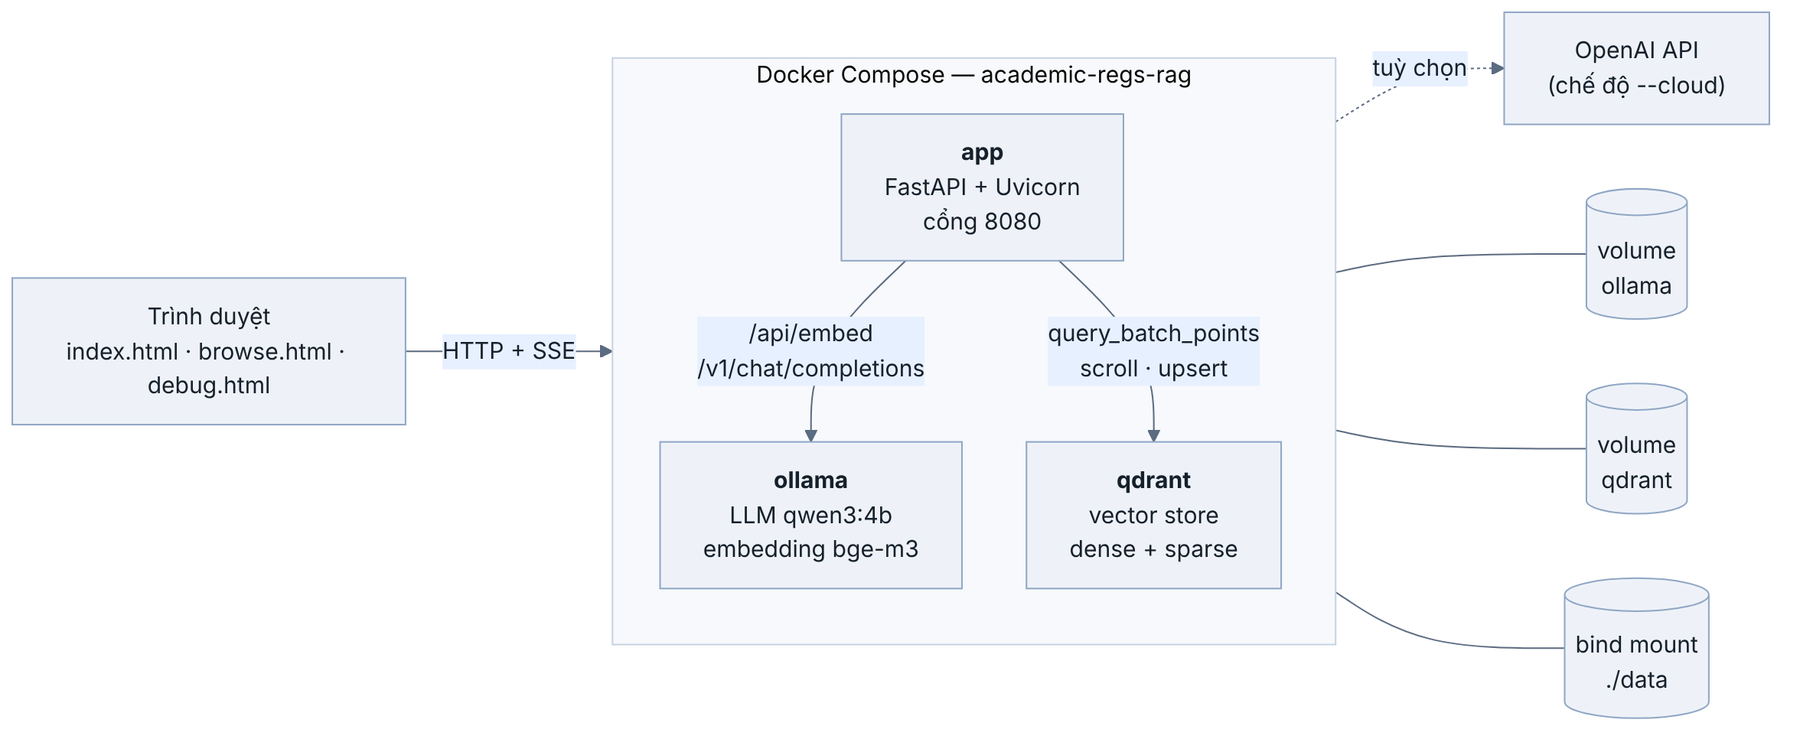
\includegraphics[width=\textwidth]{img/kien-truc.png}
\caption{Kiến trúc triển khai. Toàn bộ mô hình chạy tại chỗ; đường nét đứt tới OpenAI chỉ được
dùng khi khởi động ở chế độ \code{--cloud}, và kể cả khi đó thì embedding vẫn chạy local nên
không phải nạp lại dữ liệu.}
\label{fig:kientruc}
\end{figure}

\subsection{Các thành phần}

\begin{rtable}
\begin{tabular}{@{}p{0.17\textwidth} p{0.26\textwidth} p{0.47\textwidth}@{}}
\toprule
\tabhead{\textbf{Thành phần}} & \tabhead{\textbf{Công nghệ}} & \tabhead{\textbf{Vai trò}} \\
\midrule
\textbf{app} & FastAPI + Uvicorn, Python 3.11 &
  API HTTP, luồng SSE, pipeline truy xuất, phục vụ ba trang giao diện \\
\textbf{ollama} & Ollama, \code{qwen3:4b}, \code{bge-m3} &
  Sinh câu trả lời và tạo vector embedding, chạy hoàn toàn local \\
\textbf{qdrant} & Qdrant v1.15 &
  Lưu 90 điểm vector, mỗi điểm có một vector dense và một vector sparse \\
\textbf{Giao diện} & HTML + CSS + JavaScript thuần &
  Ba trang: hỏi đáp, tra cứu, chẩn đoán. Không framework, không CDN \\
\textbf{Dữ liệu} & bind mount \code{./data} &
  PDF gốc, Markdown đã rà soát, manifest nạp dữ liệu, log truy vấn \\
\bottomrule
\end{tabular}
\captionof{table}{Thành phần hệ thống và vai trò.}
\label{tab:thanhphan}
\end{rtable}

\subsection{Cơ sở lựa chọn công nghệ}

\begin{itemize}
  \item \textbf{Ollama thay vì gọi API đám mây.} Ràng buộc “chạy tại chỗ” là ràng buộc cứng.
  Ollama cung cấp sẵn giao diện tương thích OpenAI \cite{ollama}
  (\code{/v1/chat/completions}), nên cùng một đoạn mã khách hàng dùng được cho cả Ollama,
  OpenAI và vLLM — đổi nhà cung cấp chỉ là đổi biến môi trường.
  \item \textbf{Qdrant thay vì FAISS hay pgvector.} Qdrant hỗ trợ vector thưa có sẵn cơ chế IDF
  phía máy chủ, lọc theo trường payload, và gửi nhiều truy vấn trong một request
  (\code{query\_batch\_points}) \cite{qdrant} — ba tính năng mà pipeline này dùng trực tiếp.
  \item \textbf{bge-m3.} Đa ngôn ngữ, chất lượng tiếng Việt tốt, 1024 chiều, chạy được CPU.
  Quan trọng hơn: embedding luôn chạy local kể cả ở chế độ cloud, nên việc đổi mô hình sinh
  không bao giờ buộc phải nạp lại toàn bộ dữ liệu.
  \item \textbf{qwen3:4b.} Đủ nhỏ để chạy trên laptop, tiếng Việt chấp nhận được. Chế độ suy
  luận (“thinking”) được tắt bằng chỉ thị \code{/no\_think} vì nó làm chậm đáng kể mà không cải
  thiện chất lượng cho tác vụ tóm lược có nguồn.
  \item \textbf{Giao diện không framework.} Toàn bộ giao diện là ba file HTML và một file CSS,
  không phụ thuộc CDN. Hệ quả: hệ thống chạy được trong mạng hoàn toàn cô lập, và không có bước
  build nào giữa mã nguồn và sản phẩm.
\end{itemize}

\chapterbreak

\section{Chức năng hệ thống}

Hệ thống cung cấp 33 chức năng, chia thành bốn nhóm theo vai trò người dùng: sinh viên tra cứu,
cán bộ quản trị nội dung, và nhà phát triển tinh chỉnh hệ thống.

\subsection{Nhóm hỏi đáp}

{\sffamily\small
\begin{longtable}{@{}p{0.04\textwidth} p{0.26\textwidth} p{0.60\textwidth}@{}}
\caption{Nhóm chức năng hỏi đáp.}\label{tab:cn-hoidap}\\
\toprule
\tabhead{\textbf{\#}} & \tabhead{\textbf{Chức năng}} & \tabhead{\textbf{Mô tả}} \\
\midrule
\endfirsthead
\multicolumn{3}{@{}l}{\footnotesize\itshape Bảng \thetable{} (tiếp)}\\
\toprule
\tabhead{\textbf{\#}} & \tabhead{\textbf{Chức năng}} & \tabhead{\textbf{Mô tả}} \\
\midrule
\endhead
\bottomrule
\endlastfoot
1 & Hỏi đáp tiếng Việt có trích dẫn & Trả lời dựa hoàn toàn trên trích đoạn lấy được; mỗi ý kèm trích dẫn dạng \code{[Tên văn bản, Điều X.Y]} \\
2 & Trả lời theo luồng (streaming) & Hiển thị từng mẩu chữ ngay khi mô hình sinh ra, qua Server-Sent Events \\
3 & Hiện trích đoạn trước câu trả lời & Sự kiện \code{retrieved} gửi nguồn về trước token đầu tiên vài giây. Dòng trạng thái ghi “đang đọc N trích đoạn”, không hứa trước là chúng trả lời được \\
4 & Trích dẫn bấm được & Danh sách nguồn mặc định đóng, có nút bung kèm số lượng. Bấm vào \code{[…, Điều 5.2]} trong câu trả lời sẽ tự bung danh sách và làm nổi bật đúng trích đoạn \\
5 & Mở PDF gốc đúng trang & Nút PDF ở mỗi nguồn mở bản scan gốc tại đúng số trang chứa điều khoản đó \\
6 & Hội thoại nhiều lượt & Gửi kèm 3 lượt gần nhất làm ngữ cảnh; câu hỏi nối tiếp phụ thuộc ngữ cảnh được viết lại thành câu độc lập trước khi tra cứu \\
7 & Từ chối khi ngoài phạm vi & Từng trích đoạn phải tự vượt ngưỡng liên quan; không còn trích đoạn nào thì trả lời “không tìm thấy” kèm gợi ý các Điều gần nhất. Khi mô hình đọc trích đoạn rồi vẫn kết luận không có, giao diện nói rõ đã đọc bao nhiêu đoạn \\
8 & Cảnh báo trích dẫn vô căn cứ & Trích dẫn tới một Điều không nằm trong ngữ cảnh sẽ được tô màu cảnh báo kèm chú thích \\
9 & Sao chép \& hỏi lại & Chép nguyên văn câu trả lời; chạy lại cùng câu hỏi để so sánh hai lần sinh \\
10 & Phản hồi tốt / chưa tốt & Ghi nhận đánh giá kèm câu hỏi và nguồn đã dùng vào nhật ký, phục vụ cải thiện về sau \\
11 & Lưu hội thoại & Lưu trong trình duyệt người dùng, khôi phục sau khi tải lại trang, không gửi về máy chủ \\
12 & Dừng giữa chừng & Huỷ luồng đang sinh bằng nút Dừng hoặc phím \code{Esc}, giữ lại phần đã sinh \\
13 & Câu hỏi gợi ý & Bốn câu hỏi mẫu trên màn hình trống, bấm là hỏi ngay \\
14 & Giao diện thích ứng & Chế độ sáng/tối/theo hệ thống, bố cục chạy được trên điện thoại, phím tắt \code{/} và \code{Ctrl+K}, tôn trọng tuỳ chọn giảm chuyển động \\
\end{longtable}
}

\subsection{Nhóm tra cứu văn bản}

{\sffamily\small
\begin{longtable}{@{}p{0.04\textwidth} p{0.26\textwidth} p{0.60\textwidth}@{}}
\caption{Nhóm chức năng tra cứu văn bản.}\label{tab:cn-tracuu}\\
\toprule
\tabhead{\textbf{\#}} & \tabhead{\textbf{Chức năng}} & \tabhead{\textbf{Mô tả}} \\
\midrule
\endfirsthead
\toprule
\tabhead{\textbf{\#}} & \tabhead{\textbf{Chức năng}} & \tabhead{\textbf{Mô tả}} \\
\midrule
\endhead
\bottomrule
\endlastfoot
15 & Mục lục phân cấp & Cây Chương → Điều và danh sách Phụ lục, kèm tiêu đề và số trang, dựng trực tiếp từ chính Markdown đã được nạp nên không bao giờ lệch với dữ liệu đã đánh chỉ mục \\
16 & Lọc nhanh & Ô lọc theo số điều, tên chương hoặc từ khoá trong tiêu đề, lọc tức thời phía trình duyệt \\
17 & Đọc toàn văn một Điều & Hiển thị đầy đủ các khoản, bảng biểu được dựng lại thành bảng HTML thay vì in ra ký tự gạch đứng \\
18 & Hiển thị nguồn gốc từng khoản & Chú thích lề của bản hợp nhất (“Khoản 1, Điều 2, TT17”) được hiện kèm mỗi khoản, cho biết nội dung bắt nguồn từ văn bản gốc nào \\
19 & Mở PDF đúng trang & Liên kết tới bản scan gốc tại trang chứa điều đang đọc \\
20 & Chuyển sang hỏi đáp & Nút “Hỏi về Điều N” chuyển sang trang hỏi đáp với câu hỏi đã điền sẵn \\
\end{longtable}
}

\subsection{Nhóm chẩn đoán và vận hành}

{\sffamily\small
\begin{longtable}{@{}p{0.04\textwidth} p{0.26\textwidth} p{0.60\textwidth}@{}}
\caption{Nhóm chức năng chẩn đoán và vận hành.}\label{tab:cn-chandoan}\\
\toprule
\tabhead{\textbf{\#}} & \tabhead{\textbf{Chức năng}} & \tabhead{\textbf{Mô tả}} \\
\midrule
\endfirsthead
\toprule
\tabhead{\textbf{\#}} & \tabhead{\textbf{Chức năng}} & \tabhead{\textbf{Mô tả}} \\
\midrule
\endhead
\bottomrule
\endlastfoot
21 & Bảng điểm truy xuất & Với một câu hỏi bất kỳ, hiện từng chunk ứng viên cùng điểm fused, cosine, BM25 và điểm rerank \\
22 & So sánh thô / đầy đủ & Bật tắt để xem danh sách ứng viên thô, hoặc kết quả sau ngưỡng – rerank – mở rộng ngữ cảnh \\
23 & Hiện từ đã mở rộng & Cho biết bảng thuật ngữ đã thêm cụm nào và nhận diện được số Điều nào trong câu hỏi \\
24 & Xem cấu hình đang áp dụng & Liệt kê toàn bộ tham số truy xuất đang chạy, không chứa khoá bí mật \\
25 & Thống kê sử dụng & Tỉ lệ trả lời được, độ trễ p50/p95, số lượt trích dẫn đáng ngờ, tỉ lệ trúng cache, và danh sách câu hỏi không tìm được nội dung \\
26 & Kiểm tra sức khoẻ & Báo rõ thiếu gì: Ollama chưa chạy, model chưa tải, Qdrant chưa kết nối, hay chưa nạp dữ liệu \\
27 & Nhật ký truy vấn & Mỗi lượt một dòng JSON: câu hỏi, câu đã viết lại, số ứng viên, độ trễ, có trả lời được không \\
28 & Bộ đánh giá truy xuất & 30 câu hỏi vàng, đo recall@k / hit@final / MRR, có chế độ bật dần từng kỹ thuật và chế độ quét ngưỡng \\
29 & Bộ kiểm thử tự động & 69 test chạy được mà không cần Ollama lẫn Qdrant, nhờ Qdrant in-memory và embedder giả \\
\end{longtable}
}

\subsection{Nhóm nạp dữ liệu}

{\sffamily\small
\begin{longtable}{@{}p{0.04\textwidth} p{0.26\textwidth} p{0.60\textwidth}@{}}
\caption{Nhóm chức năng nạp dữ liệu. Ngoài PDF, pipeline nhận cả DOCX, Markdown và văn bản thuần.}\label{tab:cn-napdl}\\
\toprule
\tabhead{\textbf{\#}} & \tabhead{\textbf{Chức năng}} & \tabhead{\textbf{Mô tả}} \\
\midrule
\endfirsthead
\toprule
\tabhead{\textbf{\#}} & \tabhead{\textbf{Chức năng}} & \tabhead{\textbf{Mô tả}} \\
\midrule
\endhead
\bottomrule
\endlastfoot
30 & OCR bản scan & Nhận diện chữ tiếng Việt, tách riêng thân bài và cột chú thích lề, có bộ nhớ đệm theo mã băm của PDF \\
31 & Kiểm tra cấu trúc sau OCR & Báo các số Điều bị thiếu hoặc sai thứ tự và các chú thích lề đọc không rõ, để người rà soát biết chỗ cần xem \\
32 & Nạp dữ liệu tăng dần & Chỉ xử lý văn bản có thay đổi; văn bản bị xoá khỏi nguồn thì các chunk tương ứng cũng bị xoá khỏi Qdrant \\
33 & Nạp qua API nền & Kích hoạt nạp dữ liệu bằng một lời gọi HTTP, chạy nền, có khoá chống chạy chồng và báo trạng thái \\
\end{longtable}
}

\chapterbreak

\section{Quy trình xây dựng hệ thống}

Hệ thống được xây dựng theo bảy giai đoạn, mỗi giai đoạn tạo ra một sản phẩm kiểm chứng được
trước khi chuyển sang giai đoạn sau.

\subsection{Giai đoạn 1 — Số hoá tài liệu}

\begin{figure}[htbp]
\centering
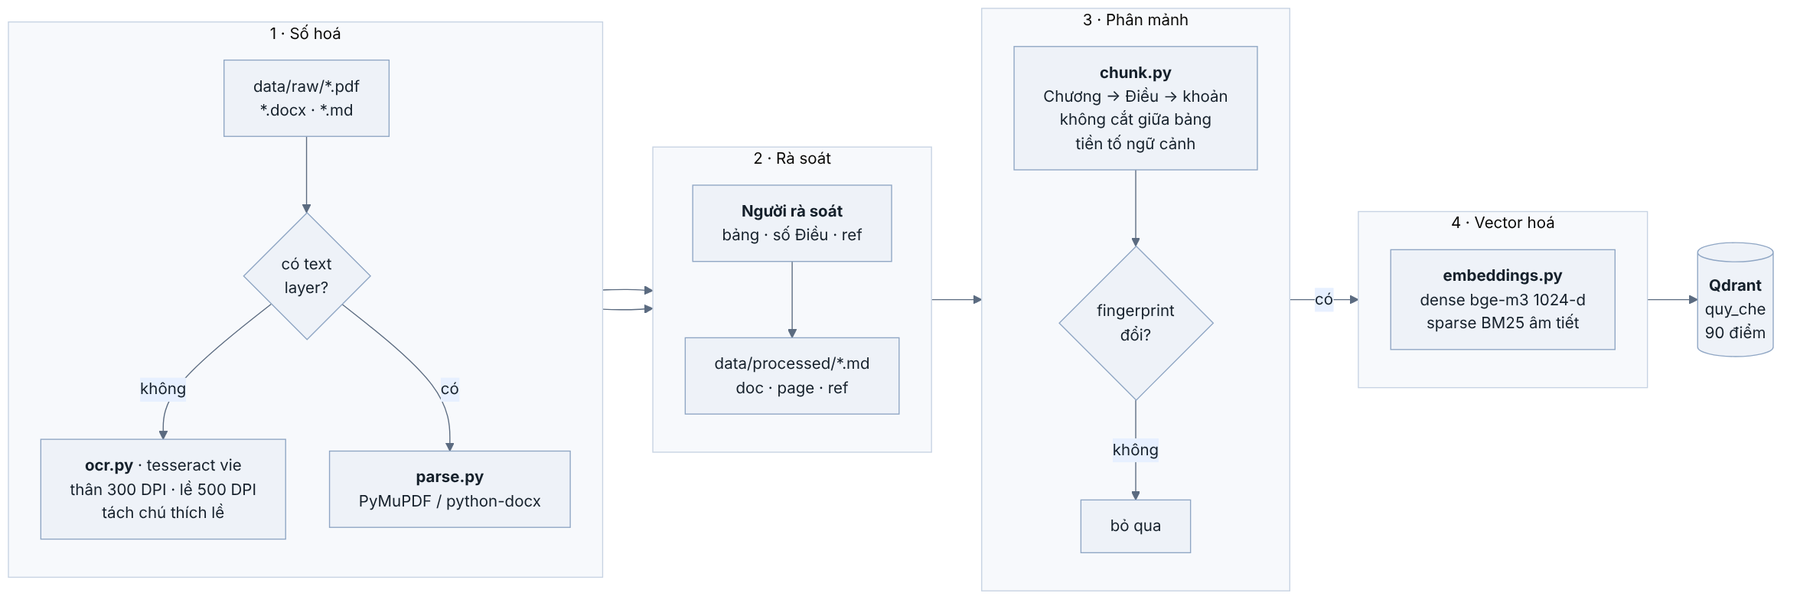
\includegraphics[width=\textwidth]{img/ingest.png}
\caption{Pipeline nạp dữ liệu, từ PDF gốc tới vector trong Qdrant. Bước rà soát của con người
là bắt buộc với bản scan và là ranh giới chất lượng của toàn hệ thống.}
\label{fig:ingest}
\end{figure}

PDF gốc là bản quét, không có lớp văn bản. Hệ thống tự phát hiện điều này (tổng số ký tự trích
được nhỏ hơn 20 ký tự mỗi trang) và chuyển sang OCR bằng Tesseract với gói ngôn ngữ tiếng Việt.
Kết quả OCR được ghi ra Markdown kèm ba loại chú thích máy đọc được:

\begin{codeblock}
<!-- doc: {"doc_id": ..., "number": "285/ĐHBK-ĐT", "effective_year": 2022} -->
<!-- page: 4 -->
<!-- ref: Khoản 3.1, Điều 3, HVu_ĐH | raw: "Khoản 3.1, / Điều 3, / HVu_ĐH" -->
Điều 5. Thời gian đào tạo
5.1 Một số khái niệm thời gian đào tạo
\end{codeblock}

Bản Markdown này sau đó được \textbf{người rà soát bằng mắt}: sửa bảng, kiểm tra số Điều, đối
chiếu chú thích lề. Đây là quyết định thiết kế có chủ ý — OCR tiếng Việt trên bản quét không
bao giờ đạt 100\%, và trong bài toán quy phạm thì một con số sai do OCR sẽ lan thành câu trả
lời sai mà không ai phát hiện. Hệ thống hỗ trợ bằng lệnh kiểm tra cấu trúc, báo các số Điều
thiếu hoặc sai thứ tự và các chú thích lề đọc không rõ.

\begin{notebox}[title={Nguyên tắc}]
Markdown đã rà soát là nguồn chân lý duy nhất. Pipeline không bao giờ ghi đè lên nó: khi PDF
nguồn thay đổi, bản OCR mới được ghi ra file \code{.md.new} để người dùng tự so sánh, chứ không
xoá công sức rà soát đã bỏ ra.
\end{notebox}

\subsection{Giai đoạn 2 — Phân mảnh theo cấu trúc}

Bản Markdown được phân tích thành cây Chương → Điều/Phụ lục → khoản, rồi đóng gói thành chunk
theo quy tắc: \textbf{một Điều là một chunk} nếu vừa ngưỡng token; nếu không vừa thì gom các
khoản liên tiếp cho tới sát ngưỡng; nếu một khoản vẫn quá dài thì cắt giữa các câu, với phần
chồng lấn nhỏ. Chi tiết thuật toán ở mục~\ref{sec:chunk}.

\subsection{Giai đoạn 3 — Vector hoá và lưu trữ}

Mỗi chunk sinh ra hai biểu diễn: vector dense 1024 chiều từ \code{bge-m3}, và vector thưa BM25
tự tính. Cả hai được lưu trong cùng một điểm Qdrant, kèm payload đầy đủ siêu dữ liệu (số Điều,
tiêu đề, danh sách khoản, trang, chú thích nguồn gốc). Việc nạp dữ liệu là \emph{idempotent}:
mã định danh của chunk sinh theo công thức tất định, và một manifest lưu dấu vân tay từng văn
bản, nên chạy lại khi không có gì đổi thì không tốn một lời gọi embedding nào.

\subsection{Giai đoạn 4 — Truy xuất}

\begin{figure}[htbp]
\centering
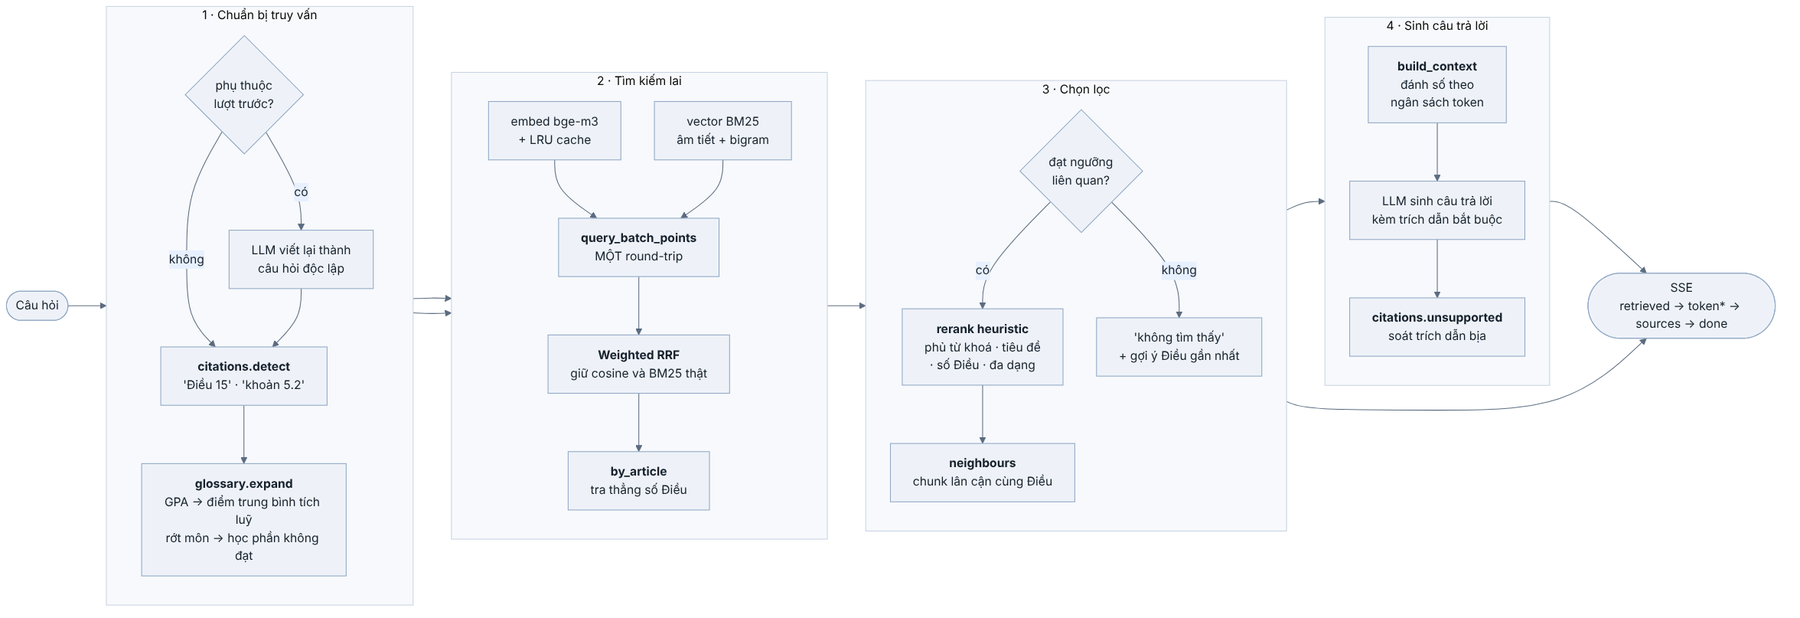
\includegraphics[width=\textwidth]{img/truy-xuat.png}
\caption{Pipeline truy xuất, bốn pha. Toàn bộ pha 1, 3 và phần hợp nhất của pha 2 là tính toán
CPU thuần; mỗi câu hỏi chỉ tốn một lời gọi tới Qdrant và một lời gọi embedding (có bộ nhớ
đệm).}
\label{fig:truyxuat}
\end{figure}

Đây là phần nhận nhiều công sức nhất của đồ án, và là phần quyết định chất lượng. Chi tiết từng
kỹ thuật được trình bày ở chương~\ref{sec:chitiet}.

\subsection{Giai đoạn 5 — Sinh câu trả lời}

Các trích đoạn được đánh số và gắn tiêu đề đầy đủ trước khi đưa vào prompt, nhờ đó mô hình
trích dẫn được tên Điều thật chứ không phải “[1]”. Prompt ràng buộc sáu quy tắc
(mục~\ref{sec:prompt}), và sau khi mô hình viết xong, mọi trích dẫn được đối chiếu ngược lại
với ngữ cảnh.

\subsection{Giai đoạn 6 — Giao diện}

\begin{figure}[htbp]
\centering
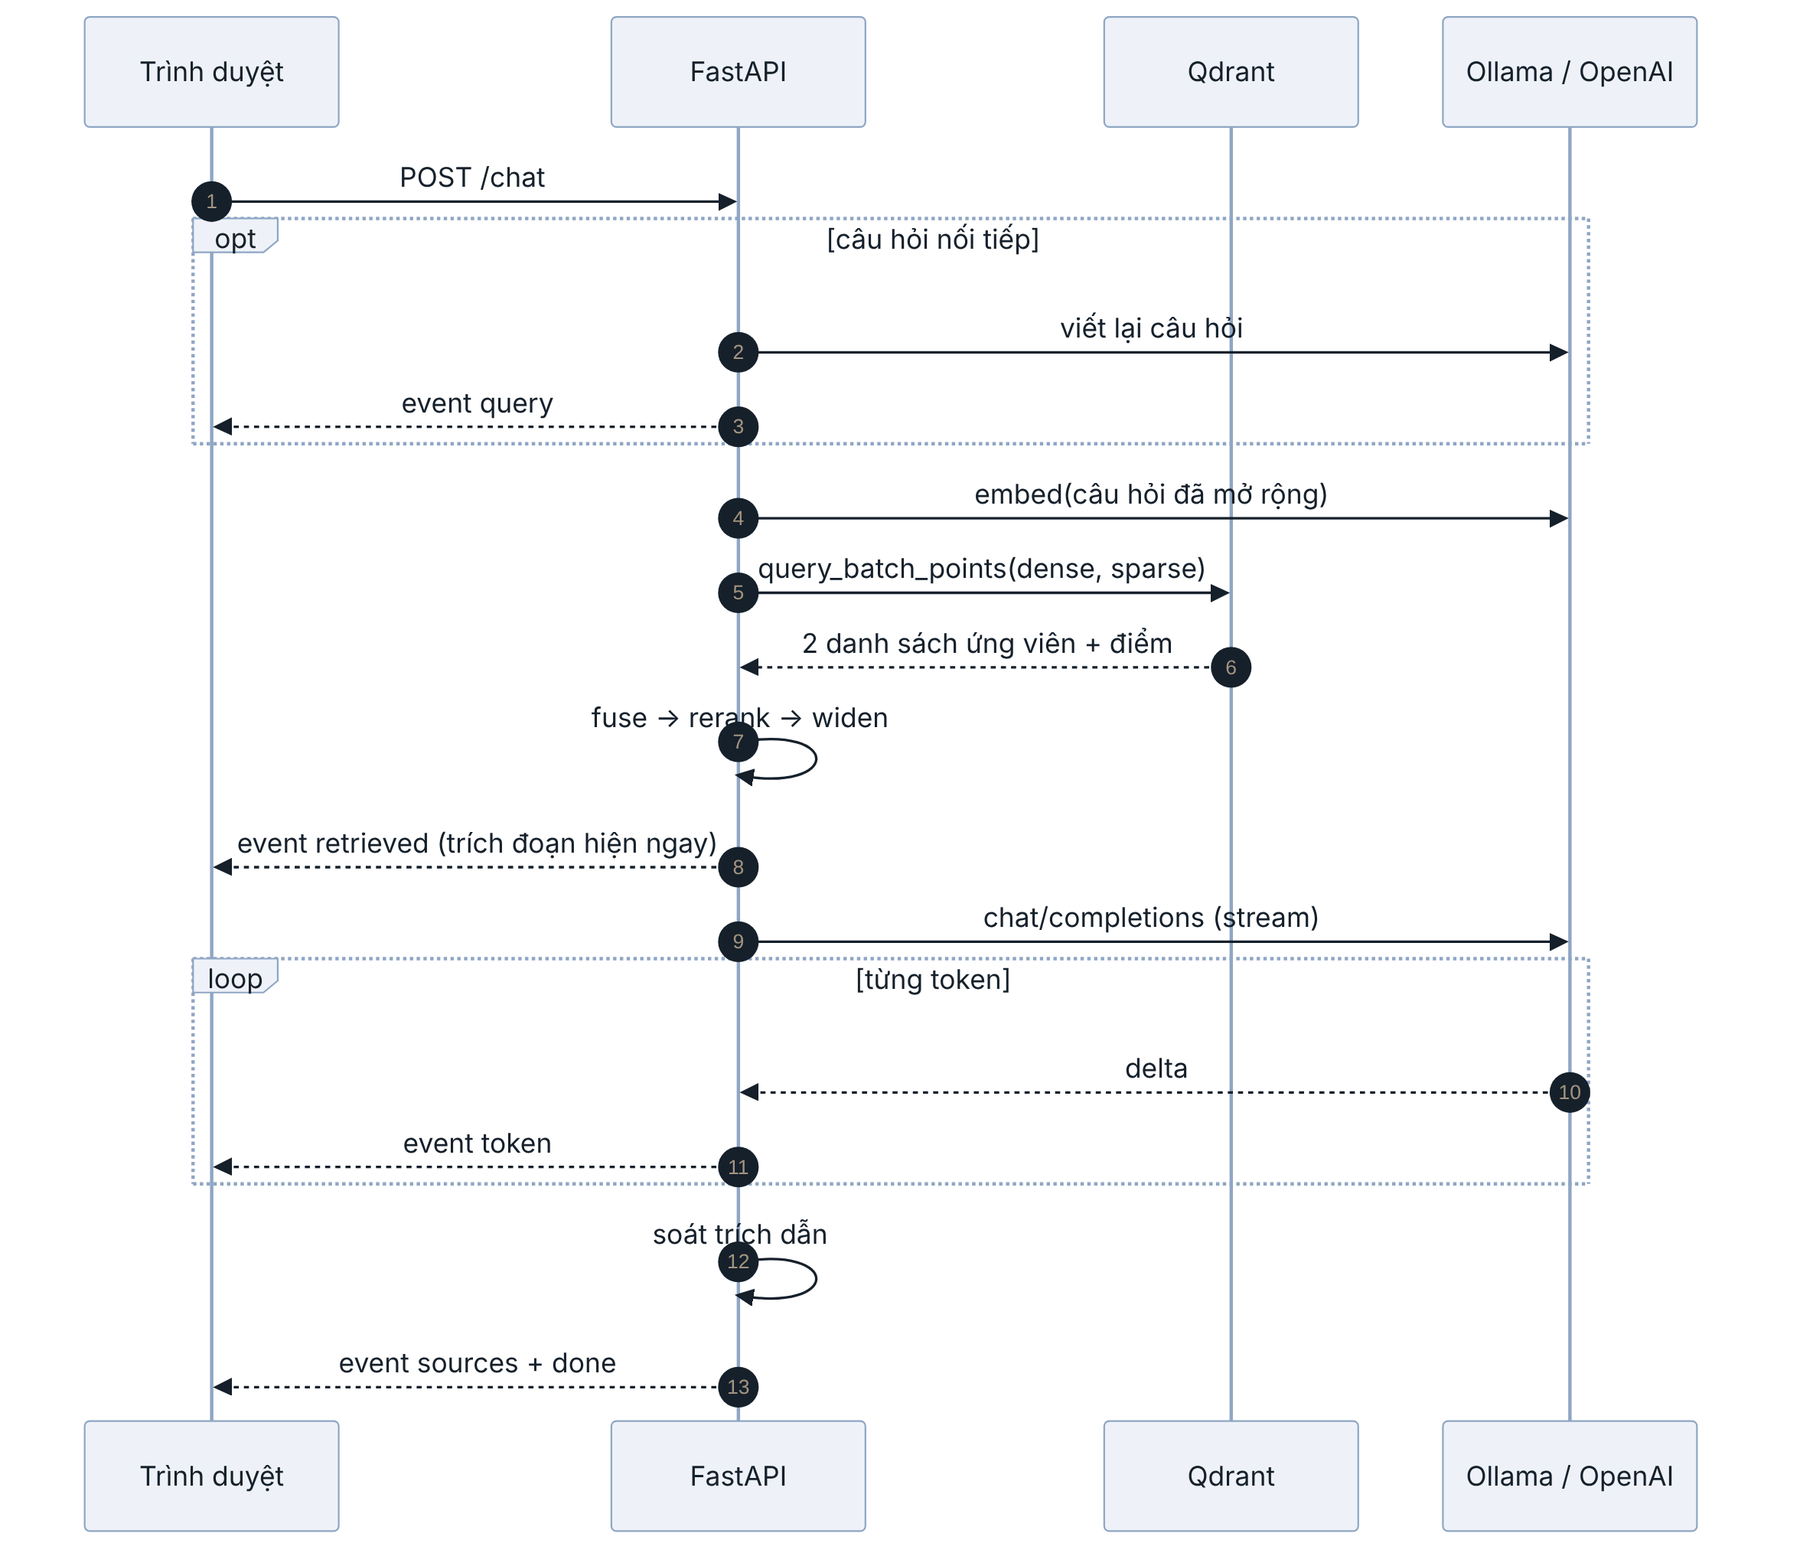
\includegraphics[width=0.78\textwidth]{img/sse.png}
\caption{Trình tự một lượt hỏi đáp. Điểm đáng chú ý là sự kiện \code{retrieved}: trích đoạn tới
trình duyệt trước khi mô hình bắt đầu viết, nên trên máy chỉ có CPU người đọc vẫn có việc để
làm ngay.}
\label{fig:sse}
\end{figure}

\subsection{Giai đoạn 7 — Kiểm thử và đánh giá}

Hai lớp kiểm chứng được xây dựng song song với hệ thống. Lớp thứ nhất là 69 test tự động chạy
trong vài giây, dùng Qdrant in-memory và một embedder băm từ vựng tất định, nên không cần
Ollama, không cần mạng, không cần GPU — điều kiện tiên quyết để bộ test thực sự được chạy
thường xuyên. Lớp thứ hai là bộ 30 câu hỏi vàng đo chất lượng truy xuất trên hệ thống thật.

\chapterbreak

\section{Chi tiết kỹ thuật}
\label{sec:chitiet}

\subsection{OCR hai độ phân giải và tách chú thích lề}

Bản hợp nhất có một cột chú thích hẹp ở lề phải ghi mỗi đoạn bắt nguồn từ văn bản gốc nào. Nếu
OCR cả trang một lượt, các chú thích này trộn vào giữa thân bài và phá vỡ cấu trúc. Giải pháp
là xử lý hai vùng riêng:

\begin{itemize}
  \item \textbf{Thân bài} dựng ở 300 DPI. Cột lề (từ 88,4\% chiều ngang trở đi) được
  \emph{xoá trắng} đúng những dải dọc có chú thích, chứ không xoá cả cột — vì một số dòng thân
  bài, như đoạn mở đầu trang 1, có tràn sang vùng đó.
  \item \textbf{Cột lề} dựng riêng ở 500 DPI vì chữ nhỏ hơn, rồi gom các dòng thành từng ghi
  chú theo khoảng cách dọc.
  \item \textbf{Khử bóng in ngược.} Bản quét hai mặt bị lộ chữ từ mặt sau; các điểm ảnh xám
  nhạt (trên ngưỡng 165) được đẩy về trắng trước khi nhận dạng.
  \item \textbf{Chuẩn hoá số.} OCR thường đọc nhầm “1” thành “l”, “I” hoặc “Ì”. Một bảng chuyển
  đổi sửa lại trước khi ghép thành chuỗi như \code{Khoản 1, Điều 2, TT17}; phần nào không chắc
  chắn được đánh dấu \code{?} để người rà soát để ý.
\end{itemize}

\subsection{Thuật toán phân mảnh}
\label{sec:chunk}

Đơn vị nhỏ nhất không bao giờ bị cắt là một \emph{block} (đoạn văn, mục gạch đầu dòng, hoặc cả
một bảng). Các block thuộc cùng một khoản tạo thành \emph{unit}; các unit thuộc cùng một
Điều/Phụ lục tạo thành một nhóm. Thuật toán đóng gói từng nhóm:

\begin{codeblock}
nếu tổng token của nhóm <= CHUNK_MAX_TOKENS:
    cả Điều là MỘT chunk                            <- trường hợp lý tưởng
ngược lại:
    gom các khoản liên tiếp cho tới sát ngưỡng
    nếu một khoản vẫn vượt ngưỡng:
        phần mở đầu ngắn (<= 150 token) được GÁN KÈM vào khoản dài phía sau
        cắt giữa các câu, chồng lấn CHUNK_OVERLAP_TOKENS
        các mảnh sau mảnh đầu được chèn lại dòng tiêu đề + " (tiếp)"
    không bao giờ kết thúc một chunk bằng một dòng tiêu đề trơ trọi
\end{codeblock}

Ba chi tiết đáng chú ý. \textbf{Thứ nhất}, câu bị ngắt bởi dấu sang trang được nối lại: nếu
block trước kết thúc không có dấu câu và block sau bắt đầu bằng chữ thường ở trang kế tiếp, hai
block được ghép. \textbf{Thứ hai}, câu dẫn vào bảng (“…được quy định như sau:”) được dính liền
với bảng, vì tách ra thì bảng mất đầu đề. \textbf{Thứ ba}, mỗi chunk mang một tiền tố ngữ cảnh
khi đem đi embed, nhưng tiền tố này \emph{không} nằm trong phần văn bản hiển thị cho người
dùng:

\begin{codeblock}
embed_text = "[Quy định học vụ ĐH (hợp nhất 2022) > Chương 2. PHƯƠNG THỨC ĐÀO TẠO
              > Điều 5. Thời gian đào tạo > 5.2 Thời gian đào tạo cụ thể]" + text
\end{codeblock}

Nhờ tiền tố này, một chunk nói về “8 học kỳ” vẫn tìm được bằng câu hỏi “thời gian đào tạo
chuẩn”, kể cả khi bản thân đoạn văn không chứa cụm đó.

\subsection{BM25 cho tiếng Việt}

Chỉ mục được xây theo \textbf{âm tiết và bigram âm tiết}: câu “đăng ký học phần” sinh ra các
term \code{đăng, ký, học, phần, đăng ký, ký học, học phần}. Bigram cho phép khớp cụm từ mà
không cần bộ tách từ tiếng Việt. Mỗi term được băm bằng BLAKE2b xuống chỉ số 31 bit; va chạm
băm hiếm và chỉ làm cộng dồn trọng số, không gây sai nghiêm trọng.

Trọng số lưu trong vector là phần tần suất của công thức BM25; thành phần IDF do Qdrant tự tính
nhờ cấu hình \code{modifier=IDF}, nên thêm văn bản mới không phải tính lại toàn kho. Tham số
\code{avgdl} được đo từ chính kho dữ liệu lúc nạp (372 âm tiết mỗi chunk) thay vì gán cứng —
con số gán cứng ban đầu là 400, lệch đáng kể và làm lệch phần chuẩn hoá độ dài.

\subsection{Mở rộng thuật ngữ}

Bảng tra gồm 38 từ viết tắt và 46 cụm thông dụng, ánh xạ sang đúng thuật ngữ trong quy định.
Cụm tương ứng được \emph{nối thêm} vào câu hỏi chứ không thay thế, nên ý gốc được giữ nguyên:

\begin{codeblock}
"GPA thấp bao nhiêu thì bị đuổi học?"
  -> "GPA thấp bao nhiêu thì bị đuổi học? — điểm trung bình tích luỹ; buộc thôi học"
\end{codeblock}

Ba cơ chế khớp. Viết tắt từ 3 ký tự trở lên khớp không phân biệt hoa thường; viết tắt 2 ký tự
(\code{TC}, \code{HK}, \code{HP}) bắt buộc viết hoa, để “tc” trong văn bản thường không bị hiểu
nhầm. Cụm thông dụng khớp không phân biệt hoa thường, ưu tiên cụm dài hơn (“bằng hai” thắng
“bằng”). Và khi phát hiện câu hỏi \textbf{không có dấu}, hệ thống đối chiếu bản không dấu của
câu hỏi với bản không dấu của bảng tra để khôi phục những cụm nhận ra được.

\subsection{Tra cứu trực tiếp theo số điều}

Khi câu hỏi gọi tên một điều khoản — “Điều 15 nói gì?”, “khoản 5.2 quy định sao?”, “phụ lục 7”
— ý định của người dùng là tường minh, và việc trông chờ hai vector đồng ý với nhau là thừa rủi
ro. Hệ thống nhận diện mẫu này bằng biểu thức chính quy (có xử lý số 0 đứng đầu và lỗi chính tả
dấu), rồi lấy thẳng các chunk của điều đó từ Qdrant qua bộ lọc payload, ghép vào danh sách ứng
viên. Các chunk này còn được cộng điểm thưởng lớn nhất trong bước rerank, và bỏ qua cả ngưỡng
liên quan.

\subsection{Hợp nhất có trọng số trong một round-trip}
\label{sec:fusion}

Phiên bản đầu dùng \code{FusionQuery(RRF)} của Qdrant. Vấn đề: RRF chỉ trả về điểm theo thứ
hạng, trong khi ngưỡng liên quan cần cosine thật — nên phải gọi Qdrant \emph{lần thứ hai} chỉ
để lấy lại cosine của đúng những điểm vừa tìm được. Hai round-trip cho một câu hỏi.

Phiên bản hiện tại gửi hai nhánh trong \textbf{một} request (\code{query\_batch\_points}), rồi
hợp nhất bằng Python:

\[
\mathrm{fused}(d) \;=\; \frac{w_{\text{dense}}}{60 + \mathrm{rank}_{\text{dense}}(d)}
\;+\; \frac{w_{\text{sparse}}}{60 + \mathrm{rank}_{\text{sparse}}(d)}
\]

với $w_{\text{dense}} = 1{,}0$ và $w_{\text{sparse}} = 0{,}8$ (dense được tin hơn một chút vì
các term BM25 bị băm). Điểm cosine và điểm BM25 gốc của từng nhánh được giữ nguyên trên mỗi ứng
viên, phục vụ ngưỡng liên quan, bộ rerank và trang chẩn đoán.

\subsection{Rerank heuristic}
\label{sec:rerank}

Bộ rerank chấm lại ứng viên bằng những tín hiệu mà tìm kiếm vector bỏ qua:

\begin{rtable}
\begin{tabular}{@{}p{0.32\textwidth} r p{0.47\textwidth}@{}}
\toprule
\textbf{Tín hiệu} & \textbf{Trọng số} & \textbf{Lý do} \\
\midrule
Điểm hợp nhất (chuẩn hoá) & 1,00 & Nền tảng, giữ kết quả của bước trước \\
Độ phủ từ khoá trong thân chunk & 0,45 & IDF cục bộ: từ có mặt ở mọi ứng viên thì không phân biệt được gì \\
Độ phủ trong tiêu đề Điều/Chương & 0,35 & “Điều 28. Phúc tra…” gần như chắc chắn trả lời câu hỏi về phúc tra \\
Câu hỏi gọi đúng số điều & 1,20 & Ý định tường minh phải thắng \\
Phạt trùng Điều (luỹ tiến) & $-0{,}18\,\tfrac{n(n+1)}{2}$ & Đoạn thứ hai cùng Điều vẫn cạnh tranh, đoạn thứ tư thì phải thật xuất sắc \\
\bottomrule
\end{tabular}
\captionof{table}{Tín hiệu và trọng số của bộ rerank heuristic.}
\label{tab:rerank}
\end{rtable}

\textbf{IDF cục bộ} là điểm mấu chốt: thay vì cần thống kê toàn kho, trọng số của một từ được
tính ngay trên tập ứng viên vừa lấy về, theo $\log\!\left(1 + \frac{n}{1+df}\right)$. Từ “sinh
viên” xuất hiện ở cả 20 ứng viên nên gần như không có trọng số; từ “phúc tra” xuất hiện ở một
ứng viên thì quyết định toàn bộ.

\begin{notebox}[title={Chi tiết dễ sai}]
Chuẩn hoá điểm phải \textbf{chia cho giá trị lớn nhất}, không dùng min–max. Min–max luôn ánh xạ
ứng viên tốt nhất về 1 và kém nhất về 0, nên hai ứng viên 0,51 và 0,50 trông xa nhau y như 1,0
và 0,0 — và khi đó không tín hiệu nào khác đủ sức lay chuyển thứ tự nữa. Lỗi này được phát hiện
nhờ một unit test, không phải nhờ đọc lại code.
\end{notebox}

\subsection{Mở rộng ngữ cảnh lân cận}

Câu trả lời của quy chế thường nằm vắt giữa hai khoản liền nhau: hỏi về số tín chỉ tối thiểu
thì khoản 15.3 nêu con số còn 15.4 nêu ngoại lệ. Sau khi chốt top-k, hệ thống lấy thêm tối đa 2
chunk lân cận trong cùng Điều và \textbf{xếp chúng xuống cuối} — vì \code{build\_context} cắt
theo ngân sách token từ cuối lên, nên phần bổ sung là thứ bị bỏ đầu tiên khi chật chỗ. Giao
diện đánh dấu riêng các đoạn này bằng nhãn “ngữ cảnh bổ sung”.

\subsection{Ngưỡng liên quan theo từng trích đoạn}
\label{sec:nguong}

Phiên bản đầu dùng ngưỡng liên quan như một cánh cổng chung: \emph{nếu có bất kỳ} ứng viên nào
vượt \code{MIN\_RELEVANCE\_SCORE} thì toàn bộ top-k được giữ. Hệ quả là mọi câu trả lời đều kèm
đúng \code{TOP\_K\_FINAL} “nguồn tham khảo” bất kể câu hỏi thật sự cần một hay năm, và một câu
hỏi không ai trả lời được vẫn dẫn ra năm trích đoạn — ngay trước khi mô hình tuyên bố nó không
tìm thấy gì.

Hiện tại mỗi trích đoạn phải tự vượt hai ngưỡng:

\[
\text{sàn} \;=\; \max\big(\text{\code{MIN\_RELEVANCE\_SCORE}},\;
\text{cosine}_{\max} \times \text{\code{RELATIVE\_CUTOFF}}\big)
\]

Ngưỡng tương đối là phần quan trọng. Cosine của \code{bge-m3} nằm trong một dải hẹp và cao —
một đoạn văn bất kỳ vẫn đạt khoảng 0,45 — nên chỉ riêng ngưỡng tuyệt đối không tách được đoạn
đúng khỏi đoạn đệm. Ngưỡng tương đối so sánh trong phạm vi chính lần tìm kiếm đó, nên nó thích
ứng theo từng câu hỏi.

Hai ngoại lệ có chủ ý: chunk được lấy vì câu hỏi gọi đích danh số điều thì giữ bất kể điểm, và
chunk chỉ do nhánh BM25 tìm ra thì không có cosine để chấm nên chỉ xét theo thứ hạng.
\code{TOP\_K\_FINAL} trở thành \emph{trần} chứ không phải định mức, và các chunk ngữ cảnh lân
cận chỉ lấp phần chỗ trống còn lại.

\begin{notebox}[title={Tham số phải đo, không đoán}]
\code{RELATIVE\_CUTOFF} siết quá tay sẽ loại nhầm Điều đúng. Nó không thể tinh chỉnh bằng bộ
test tự động, vì embedder giả dùng trong test có phân bố cosine trải rộng hơn \code{bge-m3}
nhiều nên cùng một tỉ lệ mang ý nghĩa khác. Harness vì vậy có chế độ \code{--sweep} chạy trên
hệ thống thật, in ra đường đánh đổi giữa số nguồn hiển thị và \code{hit@k}; quy tắc chọn là lấy
giá trị lớn nhất mà \code{hit@k} chưa suy giảm. Kết quả quét ở mục~\ref{sec:sweep}.
\end{notebox}

\subsection{Prompt}
\label{sec:prompt}

Prompt hệ thống ràng buộc sáu quy tắc: (1) chỉ dùng trích đoạn; (2) không đủ thông tin thì trả
lời đúng một câu cố định; (3) mỗi ý kèm trích dẫn lấy đúng tên văn bản và số Điều ghi ở đầu
trích đoạn; (4) giữ nguyên con số, mốc thời gian, điều kiện, và nêu rõ từng đối tượng nếu quy
định khác nhau; (5) ngắn gọn, dùng gạch đầu dòng khi nhiều ý; (6) không thêm dòng tóm tắt kiểu
“→ Đáp án: …”.

Quy tắc (2) là thứ làm cho việc từ chối trở nên \emph{phát hiện được}: câu trả lời chứa đúng
chuỗi đó thì hệ thống biết là không tìm được và không hiển thị nguồn. Quy tắc (6) cần thiết vì
mô hình nhỏ hay thêm dòng tóm tắt dù đã bị cấm; giao diện có thêm một lớp lọc chuỗi cho trường
hợp mô hình vẫn cố tình.

\subsection{Soát trích dẫn}

Sau khi mô hình viết xong, mọi cụm trong ngoặc vuông được phân tích để lấy ra số Điều/Phụ lục,
rồi đối chiếu với tập các Điều thực sự có trong ngữ cảnh. Những trích dẫn không có căn cứ được
trả về trong sự kiện \code{done} và giao diện tô màu cảnh báo. Hệ thống \textbf{không sửa} câu
trả lời — sửa tự động là thay một lỗi khó thấy bằng một lỗi khác khó thấy hơn; mục tiêu chỉ là
không để một con số bịa trông có vẻ đáng tin.

\subsection{Bảo vệ bước viết lại câu hỏi}
\label{sec:rewrite}

Câu hỏi nối tiếp phụ thuộc ngữ cảnh (“còn vừa làm vừa học thì sao?”) được viết lại thành câu
độc lập trước khi tra cứu. Cơ chế này có một chế độ hỏng nguy hiểm, phát hiện được trong quá
trình kiểm thử thực tế:

\begin{figure}[htbp]
\centering
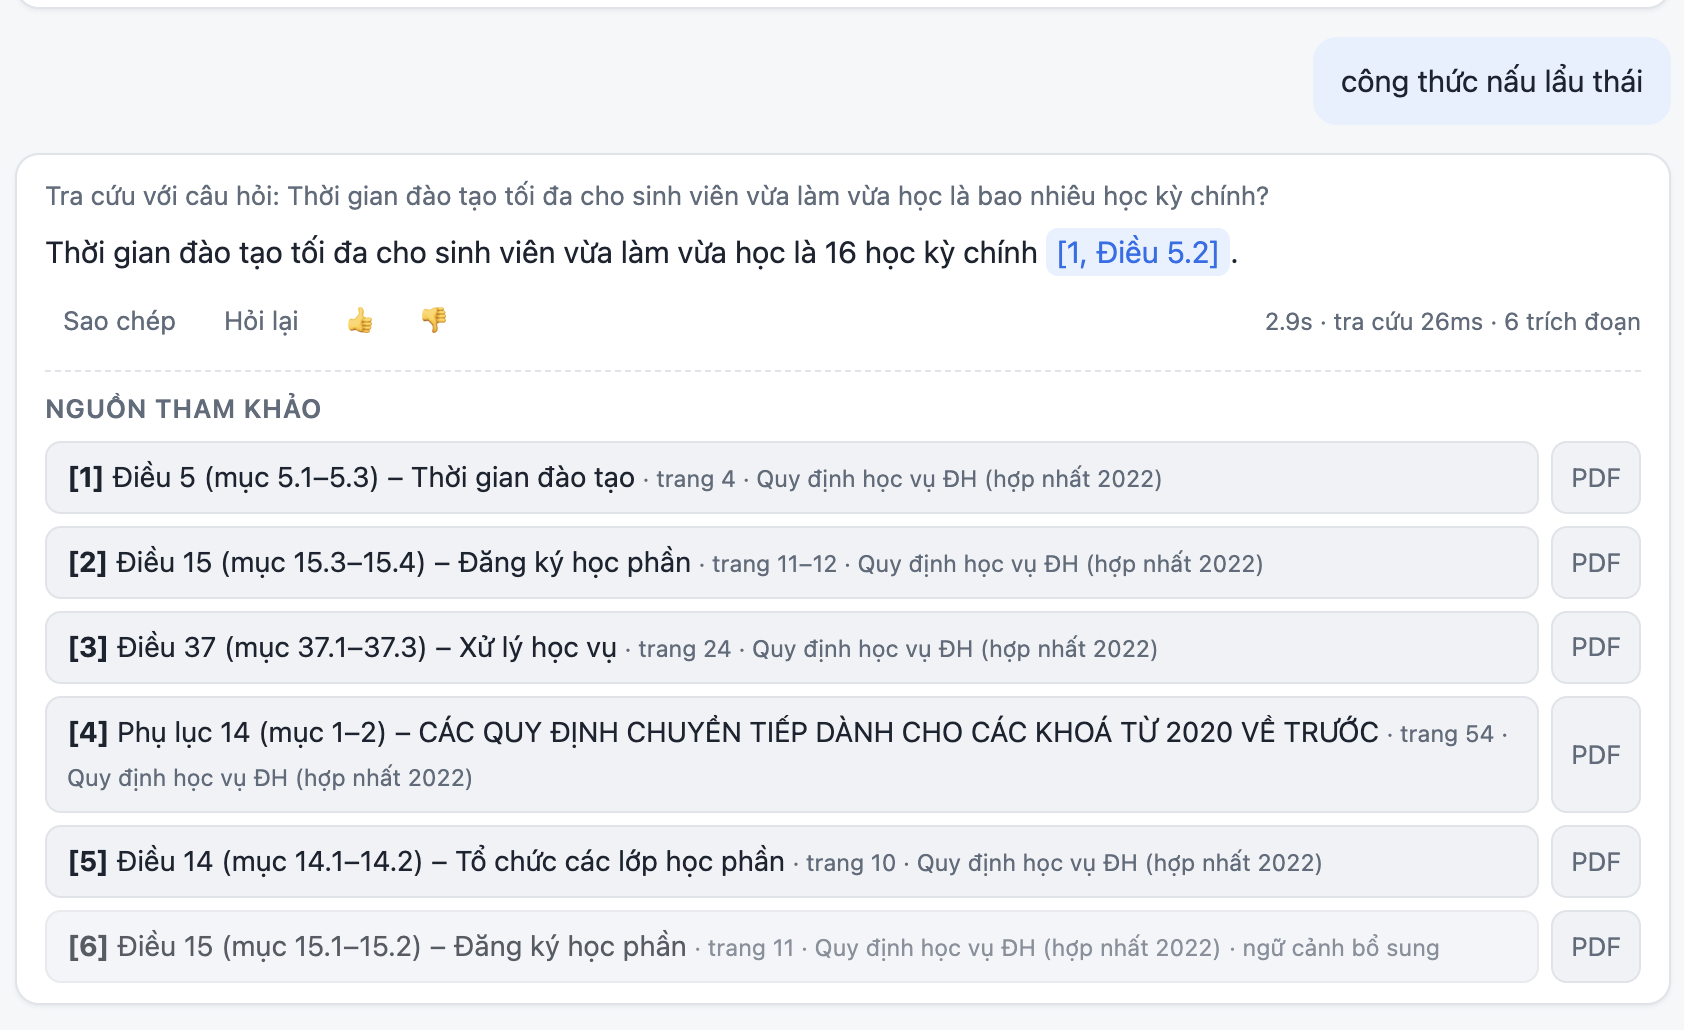
\includegraphics[width=0.88\textwidth]{img/bug-rewrite-hijack.png}
\caption{Chế độ hỏng đã được khắc phục: hỏi “công thức nấu lẩu thái” sau một lượt về thời gian
đào tạo, mô hình nhỏ trả về luôn \emph{câu hỏi trước} thay vì viết lại câu hỏi mới. Hệ quả là
câu trả lời sai chủ đề nhưng trích dẫn thật — dạng lỗi tệ nhất, vì mọi thứ phía sau đều trông
đúng.}
\label{fig:bug}
\end{figure}

Hai lớp khắc phục. Thứ nhất, ngưỡng kích hoạt được siết lại (dưới 5 từ thay vì dưới 6), nên một
câu hỏi ngắn nhưng tự đủ ý không còn bị viết lại. Thứ hai, và quan trọng hơn, kết quả viết lại
bị \textbf{kiểm tra trước khi dùng}: một bản viết lại hợp lệ luôn giữ lại ít nhất một từ nội
dung của câu hỏi gốc, vì bản chất của nó là bổ sung ngữ cảnh chứ không phải thay thế. Bản bị
cướp không giữ chữ nào của “lẩu thái” nên bị loại, hệ thống quay về câu hỏi gốc, và cơ chế
ngưỡng liên quan làm nốt phần việc từ chối.

\subsection{Nạp dữ liệu tăng dần}

Mã định danh chunk sinh bằng
\code{uuid5(doc\_id | article | index | sha256(body)[:16])} — tất định, nên nạp lại cùng một
nội dung sẽ ghi đè đúng điểm cũ chứ không nhân bản. Dấu vân tay mỗi văn bản gộp mã băm file,
phiên bản bộ phân mảnh, ngưỡng token, mô hình embedding, cờ hybrid và độ dài trung bình kho
(làm tròn theo bậc 50 âm tiết — nếu không, thêm một văn bản mới sẽ buộc nạp lại toàn bộ các văn
bản cũ chỉ vì trung bình xê dịch vài âm tiết).

\subsection{Các tối ưu độ trễ}
\label{sec:latency}

\begin{itemize}
  \item \textbf{Bỏ một round-trip Qdrant} (mục~\ref{sec:fusion}).
  \item \textbf{Bộ nhớ đệm vector câu hỏi.} Một lớp sinh viên hỏi gần như cùng vài chục câu;
  trên CPU mỗi lần embed tốn hàng chục mili-giây không cần lặp lại.
  \item \textbf{Bỏ bước viết lại khi không cần.} Trước đây \emph{mọi} câu hỏi nối tiếp đều tốn
  một lượt gọi LLM trước khi tìm kiếm.
  \item \textbf{Gửi trích đoạn trước câu trả lời.} Không làm hệ thống nhanh hơn, nhưng làm độ
  trễ \emph{cảm nhận được} ngắn hơn hẳn: người đọc có nội dung để đọc ngay.
  \item \textbf{Tắt chế độ suy luận của Qwen3} bằng \code{/no\_think}, kèm bộ lọc stream loại
  bỏ khối \code{<think>} kể cả khi thẻ bị cắt đôi giữa hai mẩu dữ liệu.
\end{itemize}

\chapterbreak

\section{Công nghệ sử dụng}

{\sffamily\small
\begin{longtable}{@{}p{0.17\textwidth} p{0.27\textwidth} p{0.46\textwidth}@{}}
\caption{Công nghệ sử dụng trong hệ thống.}\label{tab:congnghe}\\
\toprule
\textbf{Hạng mục} & \textbf{Công nghệ} & \textbf{Dùng để làm gì} \\
\midrule
\endfirsthead
\toprule
\textbf{Hạng mục} & \textbf{Công nghệ} & \textbf{Dùng để làm gì} \\
\midrule
\endhead
\bottomrule
\endlastfoot
Mô hình & bge-m3 (BAAI) & Embedding dense 1024 chiều, đa ngôn ngữ \\
        & qwen3:4b / gpt-4o-mini & Sinh câu trả lời; chế độ local hoặc cloud \\
\addlinespace
Phục vụ mô hình & Ollama & Chạy LLM và embedding local, API tương thích OpenAI \\
\addlinespace
Vector store & Qdrant v1.15 & Dense + sparse, IDF phía máy chủ, lọc payload, truy vấn theo lô \\
\addlinespace
Backend & FastAPI + Uvicorn & API HTTP, Server-Sent Events \\
        & Pydantic Settings & Cấu hình từ biến môi trường, có kiểu và giá trị mặc định \\
        & httpx & Gọi Ollama/OpenAI, hỗ trợ streaming \\
\addlinespace
Xử lý tài liệu & Tesseract OCR (gói \code{vie}) & Nhận dạng chữ tiếng Việt trên bản quét \\
        & PyMuPDF & Dựng ảnh trang, phát hiện lớp văn bản, trích văn bản \\
        & Pillow + NumPy & Khử bóng in ngược, che vùng lề trước khi OCR \\
        & python-docx & Đọc tài liệu Word \\
\addlinespace
Giao diện & HTML/CSS/JS thuần & Ba trang, không framework, không CDN, hoạt động offline \\
\addlinespace
Hạ tầng & Docker + Docker Compose & Ba dịch vụ, healthcheck, volume bền vững \\
        & Bash / PowerShell & Script khởi động một lệnh, tự dò GPU và Ollama native \\
\addlinespace
Chất lượng & pytest & 69 test, chạy không cần Ollama/Qdrant \\
        & ruff & Lint và sắp xếp import \\
        & Harness tự viết & Đo recall@k / hit@final / MRR trên bộ câu hỏi vàng \\
\end{longtable}
}

Thuật toán tự cài đặt, không dùng thư viện: BM25 cho tiếng Việt, hợp nhất RRF có trọng số,
rerank heuristic, phân mảnh bám cấu trúc, tách chú thích lề khi OCR, soát trích dẫn, trình dựng
Markdown phía trình duyệt.

\chapterbreak

\section{Demo và kết quả}

\subsection{Giao diện hỏi đáp}

\begin{figure}[htbp]
\centering
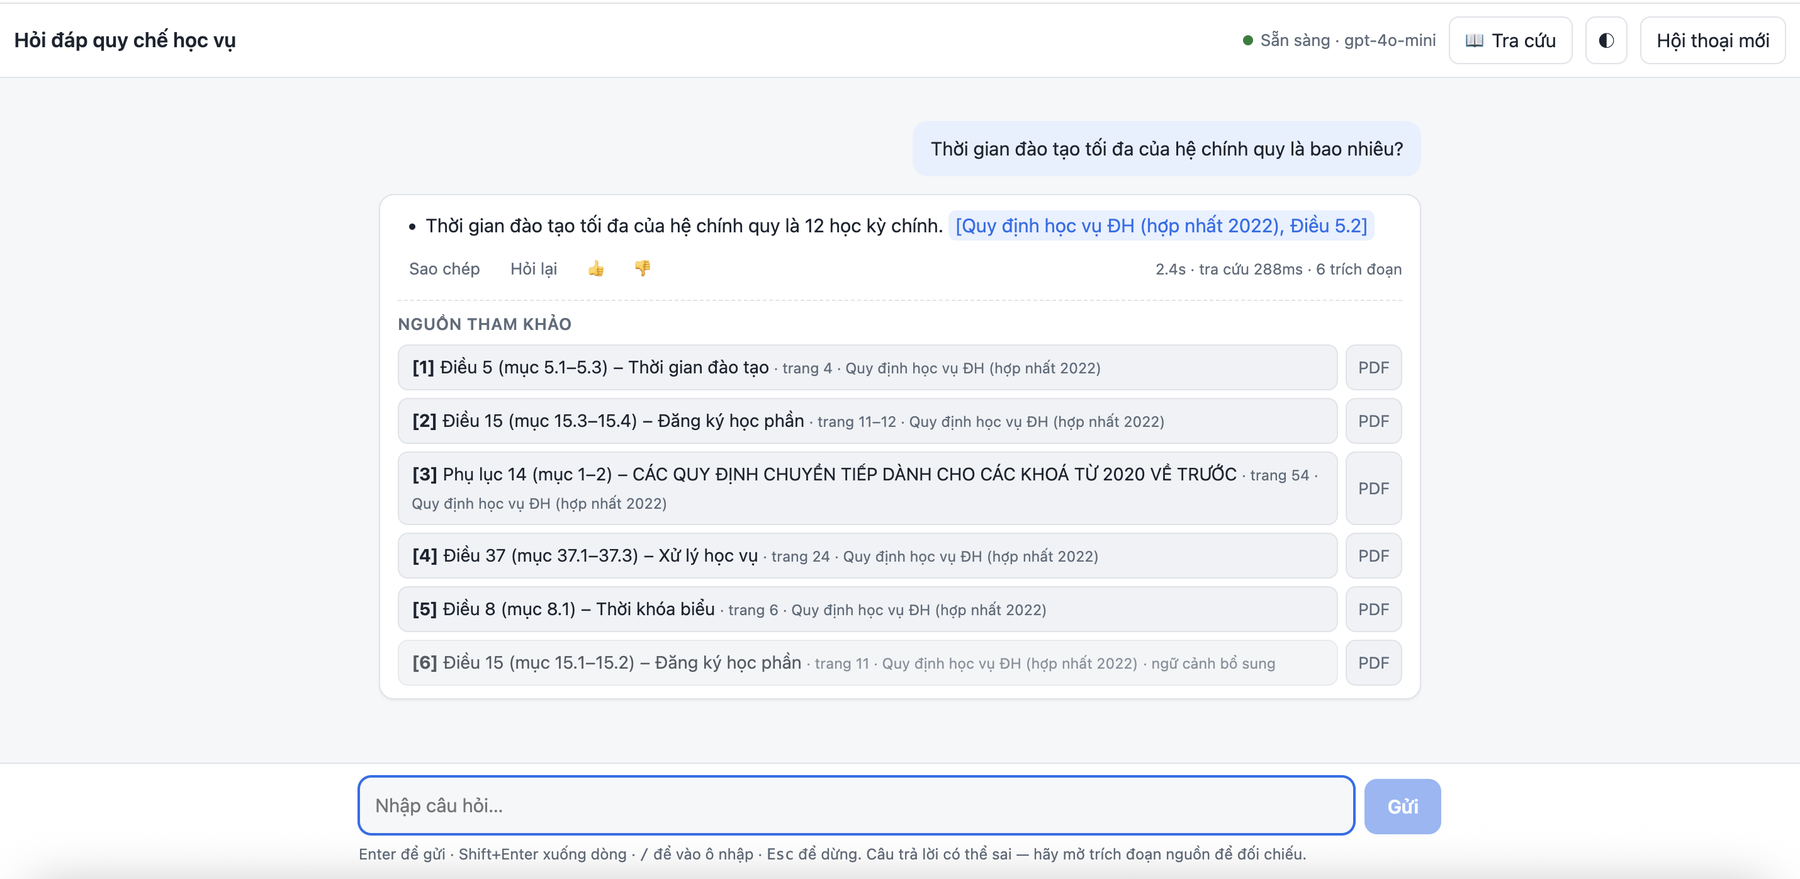
\includegraphics[width=\textwidth]{img/chat-demo.png}
\caption{Một lượt hỏi đáp. Trích dẫn \code{[Quy định học vụ ĐH (hợp nhất 2022), Điều 5.2]} được
tô nền và bấm được; dòng trạng thái cho biết tổng 2,4 giây, trong đó truy xuất 288\,ms.}
\label{fig:chat1}
\end{figure}

Câu trả lời đúng (12 học kỳ chính) và trích dẫn đúng tới khoản 5.2. Ảnh được chụp ở phiên bản
trước khi áp dụng ngưỡng liên quan theo từng trích đoạn, nên danh sách nguồn còn đủ sáu mục —
chính hiện tượng được mô tả ở mục~\ref{sec:nguong} và đã khắc phục
(xem hình~\ref{fig:count}).

\begin{figure}[htbp]
\centering
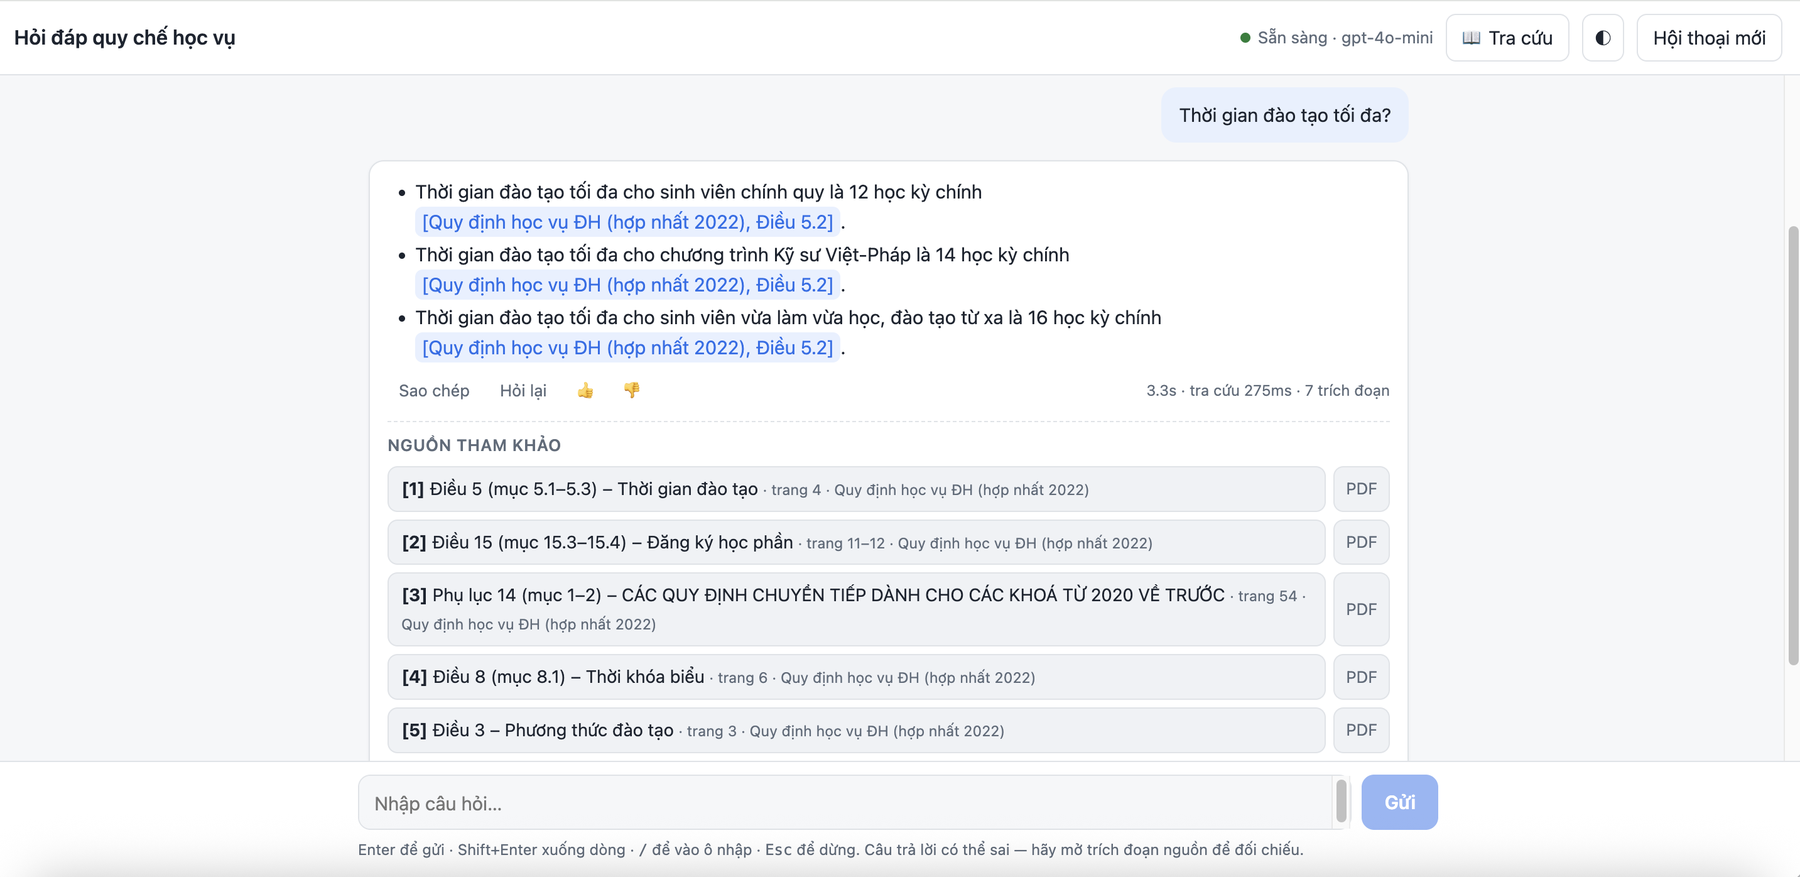
\includegraphics[width=\textwidth]{img/demo-chat-multi.png}
\caption{Khi quy định khác nhau theo đối tượng, prompt buộc mô hình nêu rõ từng trường hợp thay
vì gộp một con số: chính quy 12, Kỹ sư Việt-Pháp 14, vừa làm vừa học 16 học kỳ chính — đúng ba
dòng của bảng trong khoản 5.2.}
\label{fig:chat2}
\end{figure}

\begin{figure}[htbp]
\centering
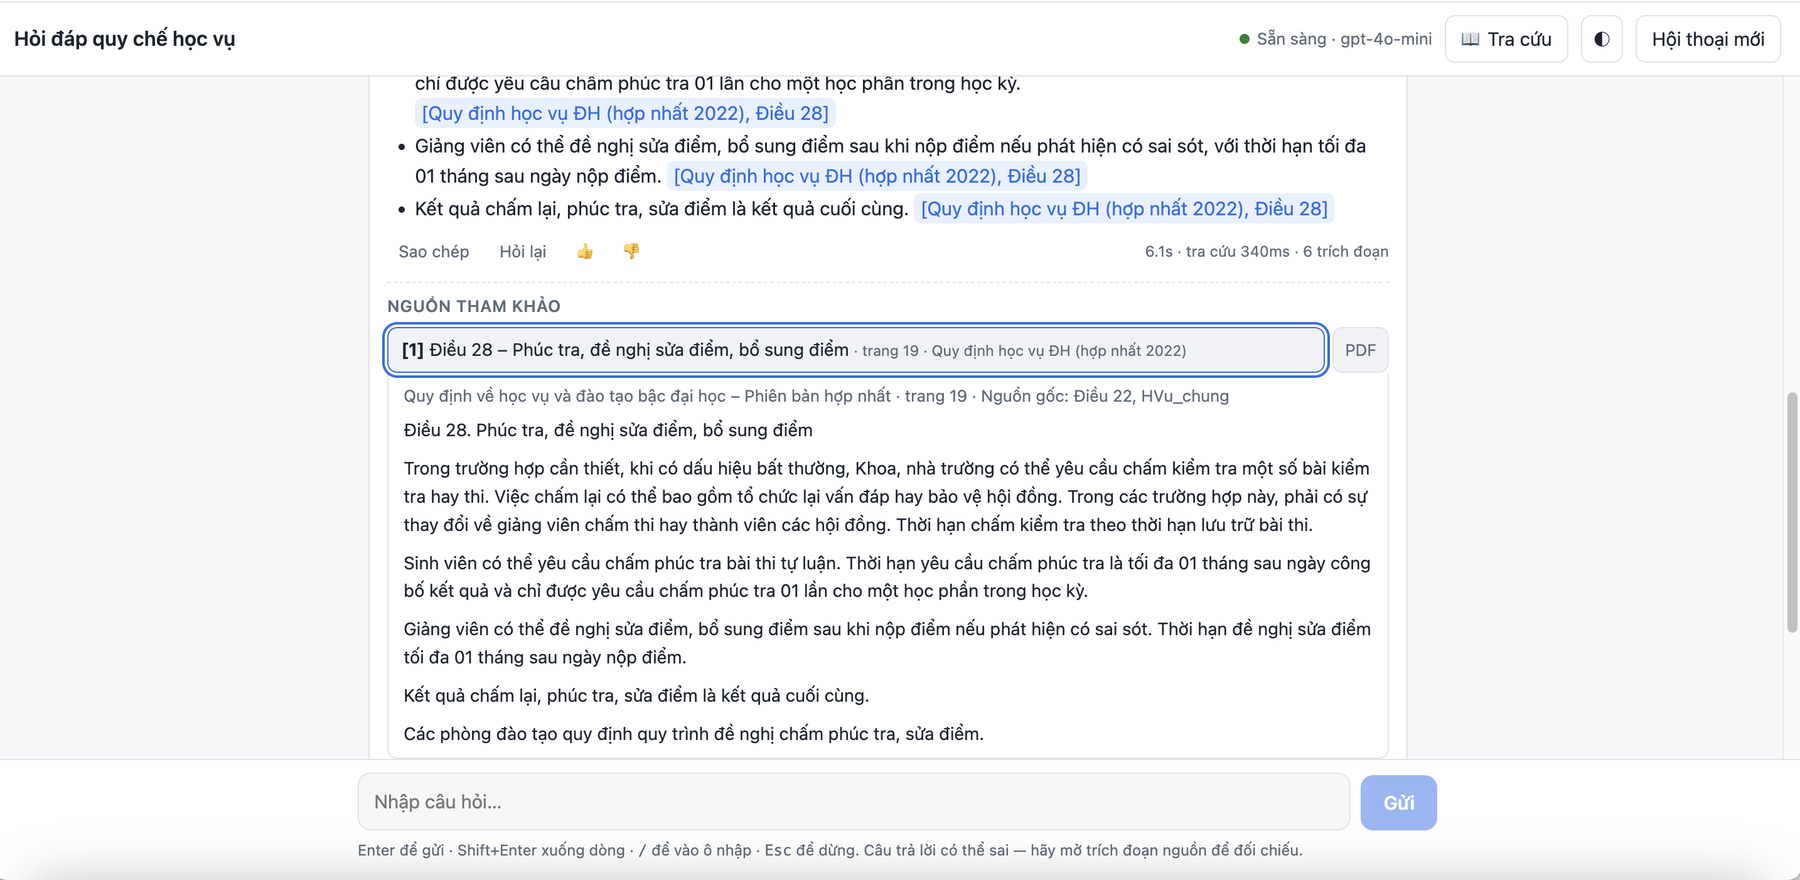
\includegraphics[width=\textwidth]{img/demo-source-open.png}
\caption{Bung một nguồn tham khảo. Toàn văn Điều 28 hiện ra kèm dòng xuất xứ “Nguồn gốc: Điều
22, HVu\_chung” — chú thích lề của bản hợp nhất, được OCR tách riêng và giữ lại suốt pipeline.
Người đọc đối chiếu được ngay mà không rời trang.}
\label{fig:source}
\end{figure}

\begin{figure}[htbp]
\centering
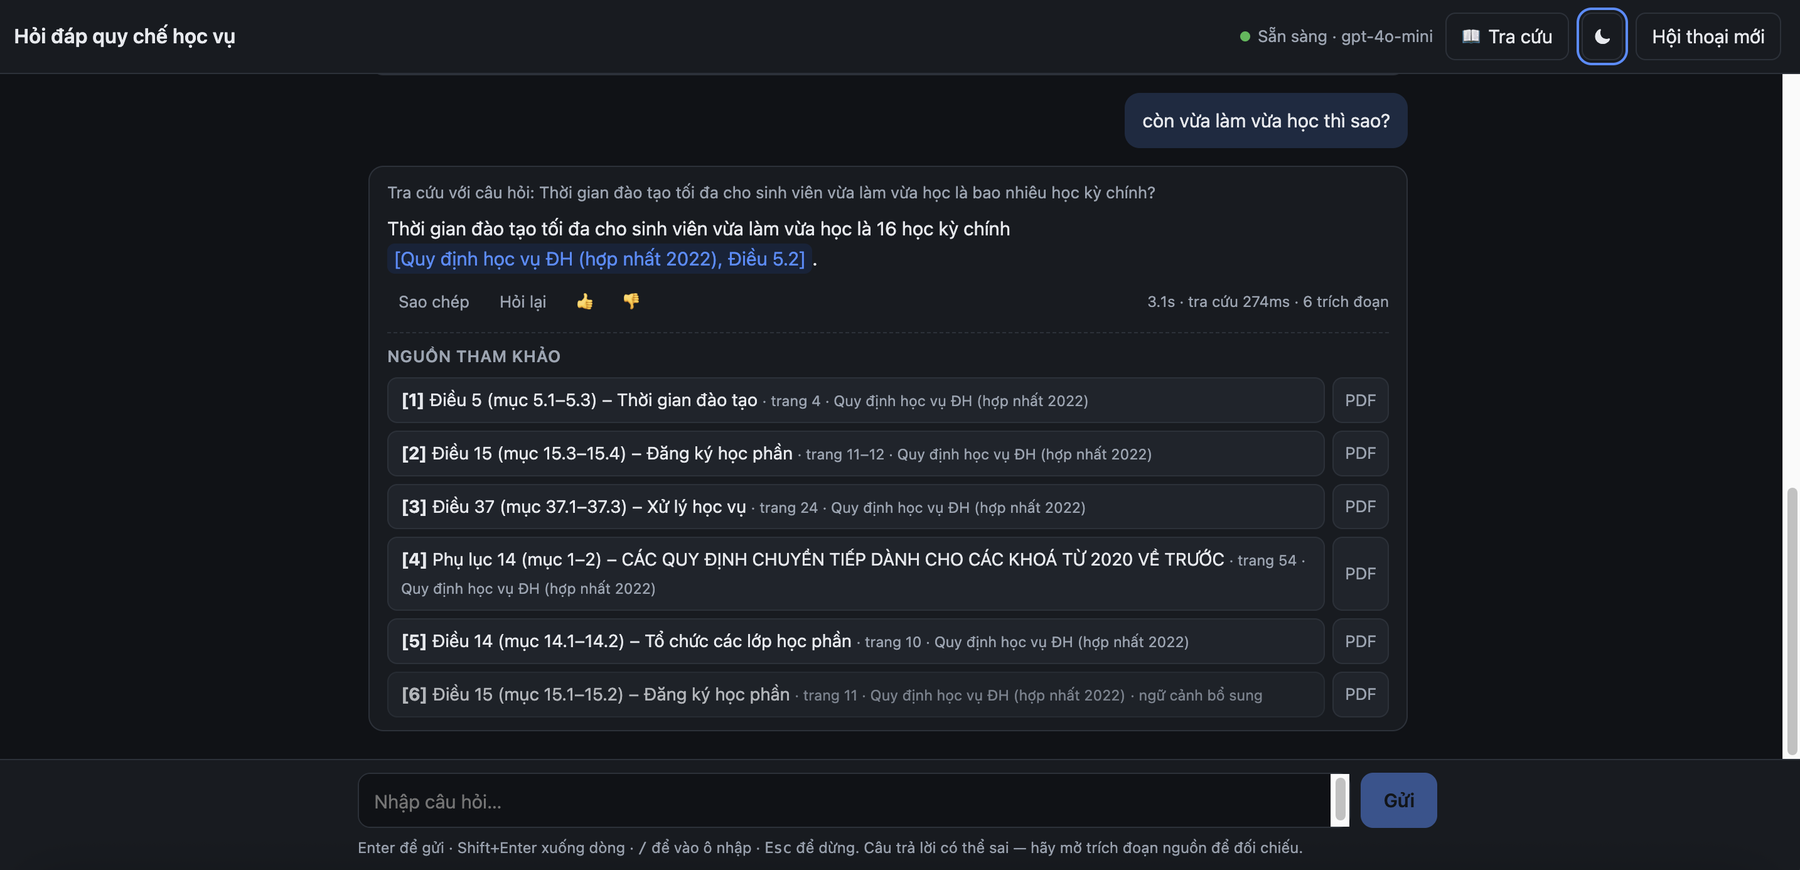
\includegraphics[width=\textwidth]{img/demo-dark-followup.png}
\caption{Câu hỏi nối tiếp “còn vừa làm vừa học thì sao?” được viết lại thành câu độc lập (dòng
xám phía trên) trước khi tra cứu, nên vẫn tìm đúng khoản 5.2 dù câu hỏi không nhắc tới thời
gian đào tạo. Ảnh cũng cho thấy chế độ giao diện tối.}
\label{fig:followup}
\end{figure}

\begin{figure}[htbp]
\centering
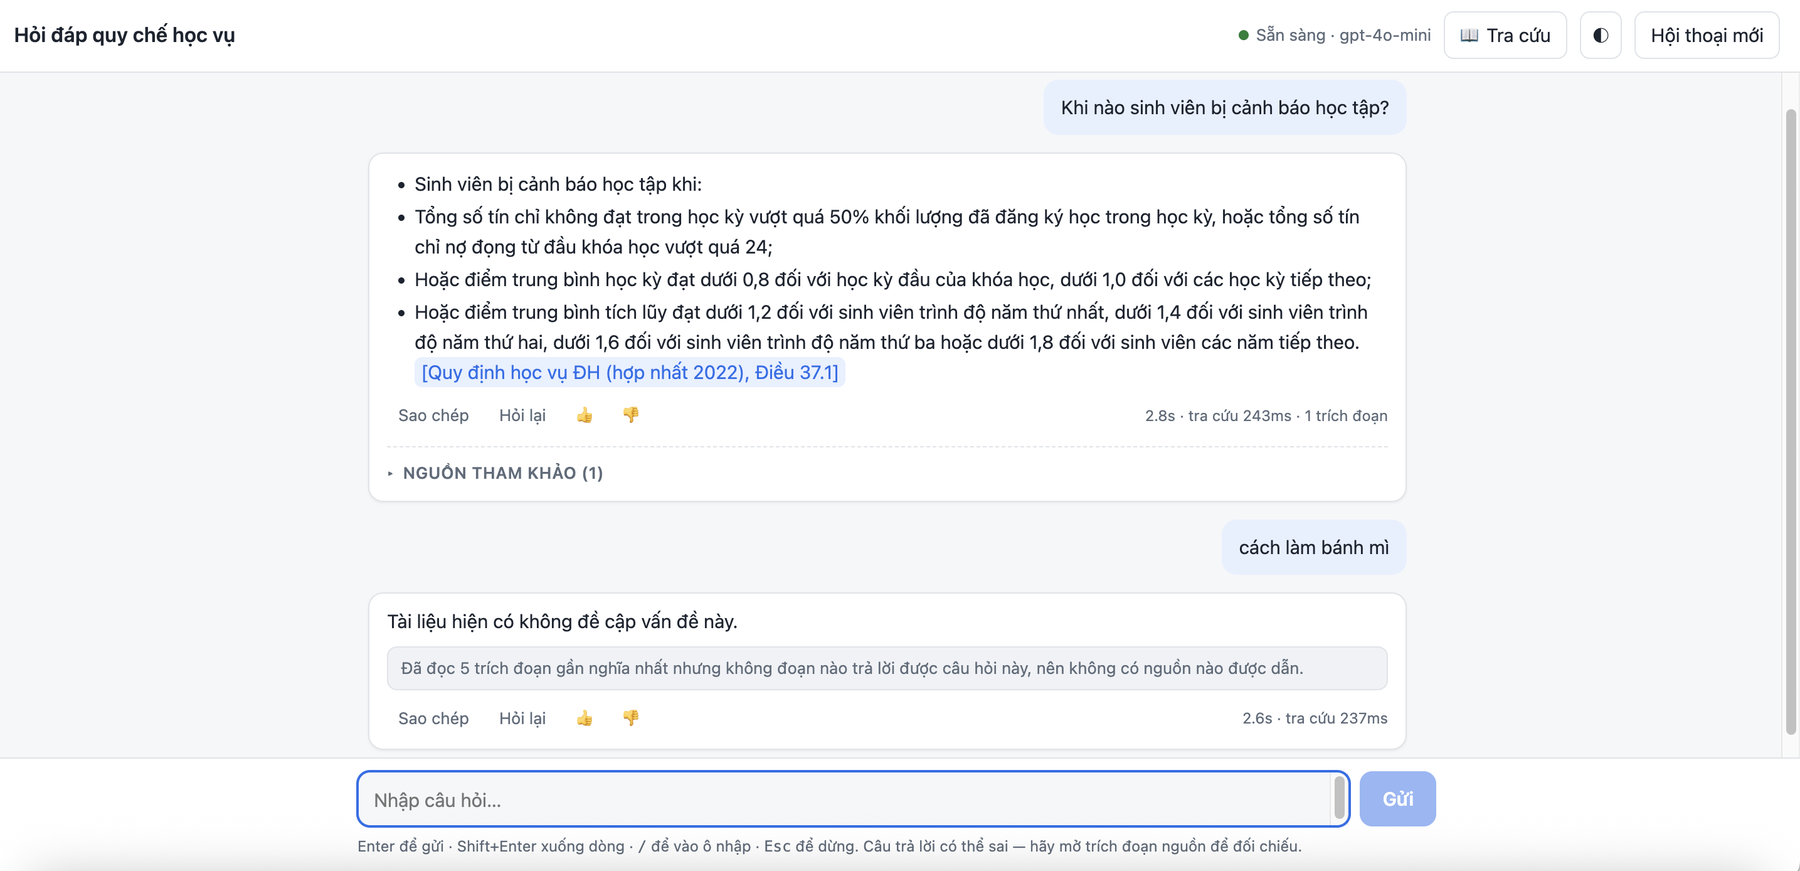
\includegraphics[width=\textwidth]{img/demo-count-refusal.png}
\caption{Hai hành vi trong một màn hình. Câu hỏi về cảnh báo học tập được trả lời bằng
\textbf{đúng một} trích đoạn, vì ngưỡng liên quan theo từng trích đoạn
(mục~\ref{sec:nguong}) đã loại phần còn lại. Câu hỏi ngoài phạm vi phía dưới nhận một lời từ
chối, kèm dòng giải thích đã đọc bao nhiêu trích đoạn và vì sao không dẫn nguồn nào.}
\label{fig:count}
\end{figure}

\begin{figure}[htbp]
\centering
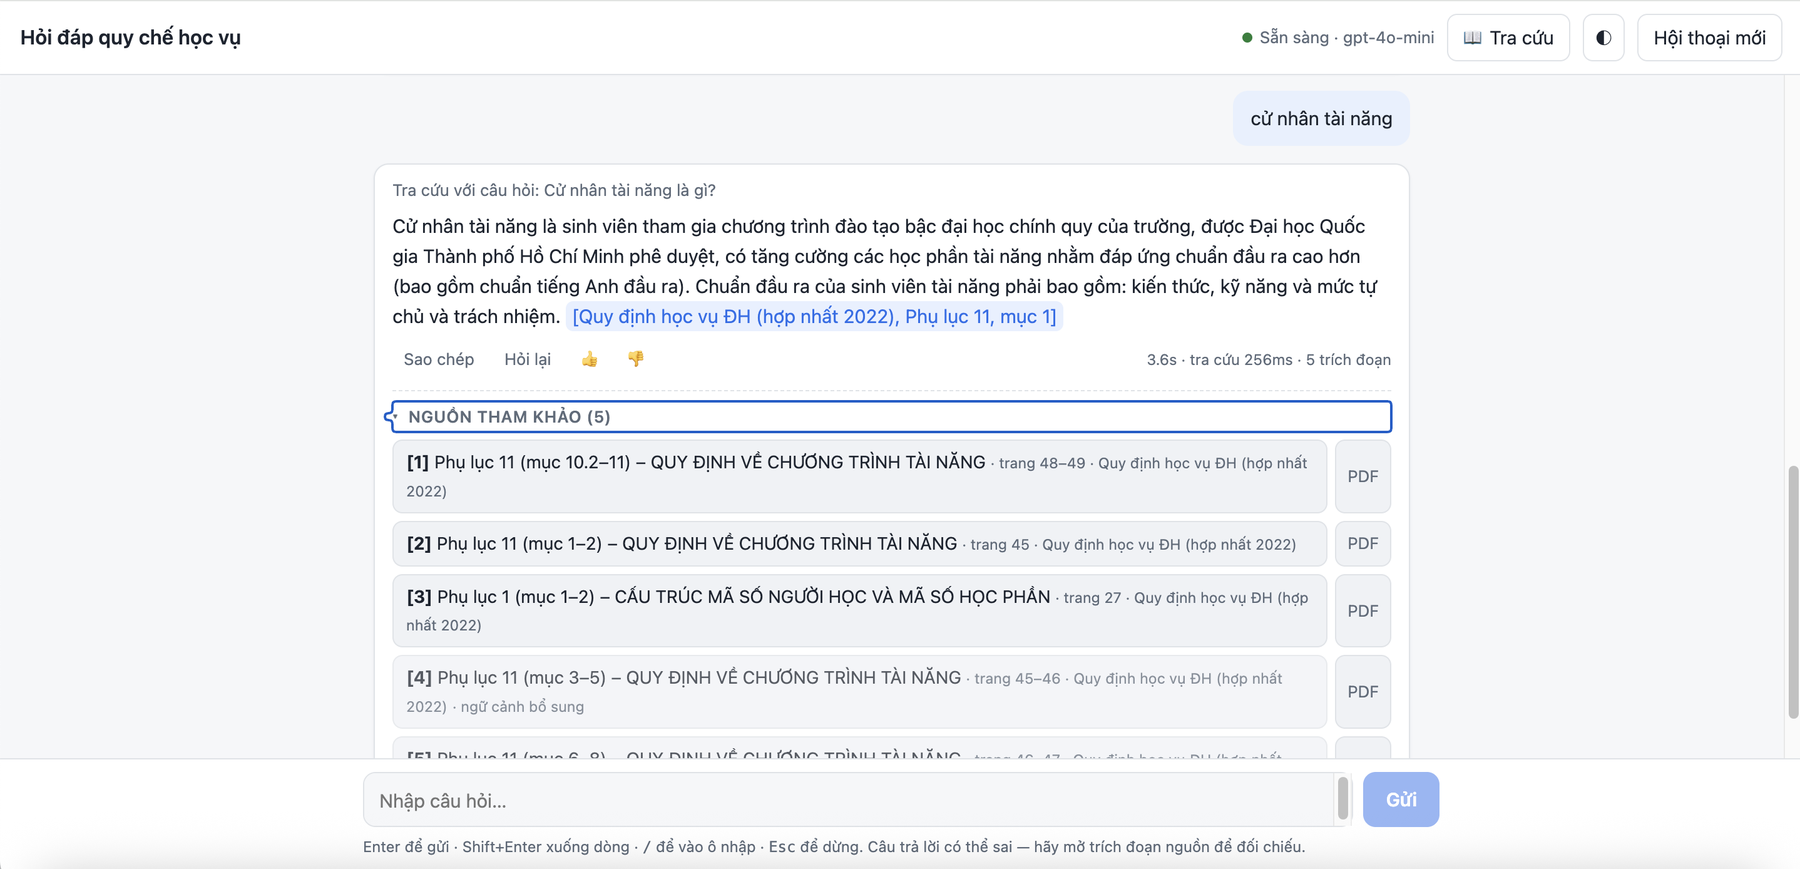
\includegraphics[width=\textwidth]{img/demo-sources-open-5.png}
\caption{Cùng giao diện, câu hỏi rộng hơn: năm trích đoạn vượt ngưỡng, và người đọc đã bấm bung
danh sách. Trích dẫn trỏ tới một Phụ lục thay vì một Điều, và câu hỏi hai từ “cử nhân tài năng”
được viết lại thành câu hoàn chỉnh trước khi tra cứu.}
\label{fig:open5}
\end{figure}

\subsection{Trang tra cứu toàn văn}

\begin{figure}[htbp]
\centering
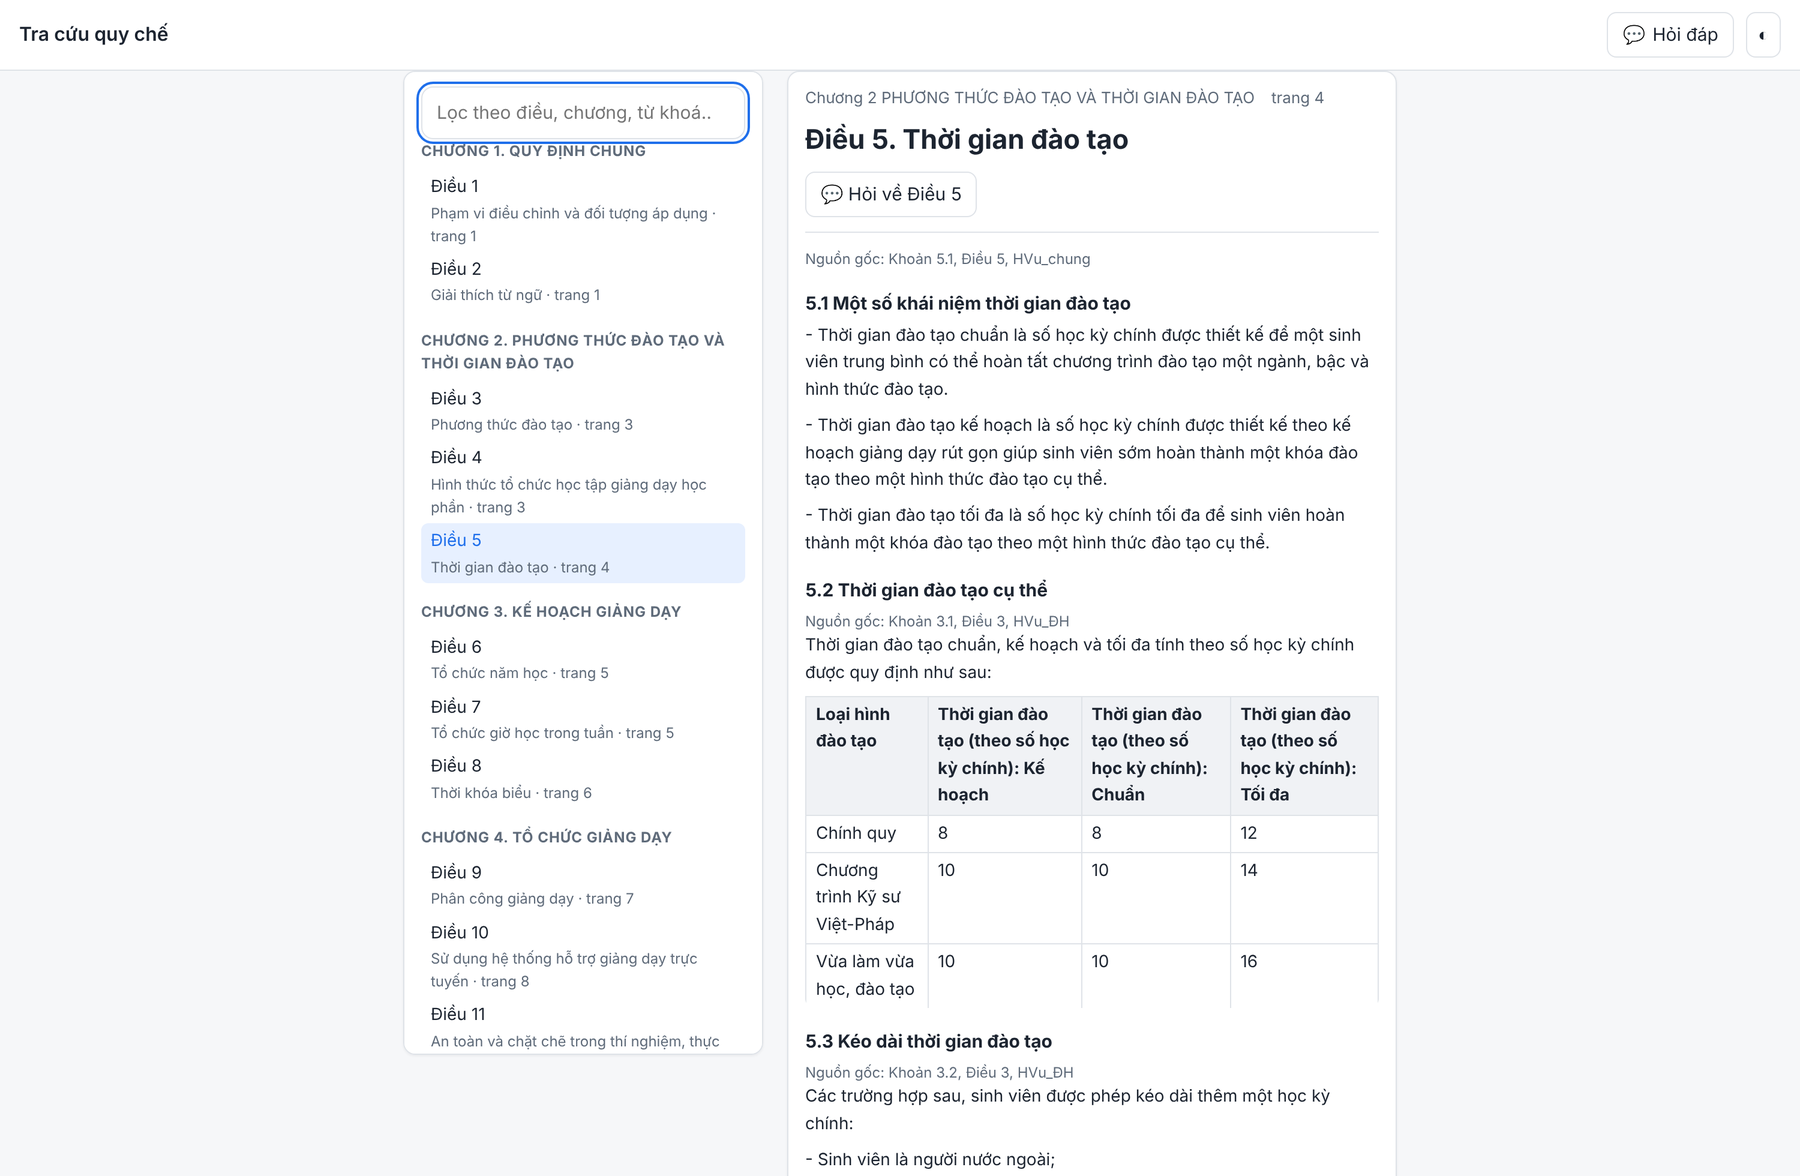
\includegraphics[width=\textwidth]{img/browse-dieu5.png}
\caption{Trang tra cứu. Mục lục bên trái dựng trực tiếp từ Markdown đã được nạp nên không bao
giờ lệch với dữ liệu đã đánh chỉ mục. Bảng “thời gian đào tạo” được dựng lại thành bảng HTML,
và mỗi khoản hiện chú thích nguồn gốc riêng.}
\label{fig:browse}
\end{figure}

\subsection{Trang chẩn đoán truy xuất}

\begin{figure}[htbp]
\centering
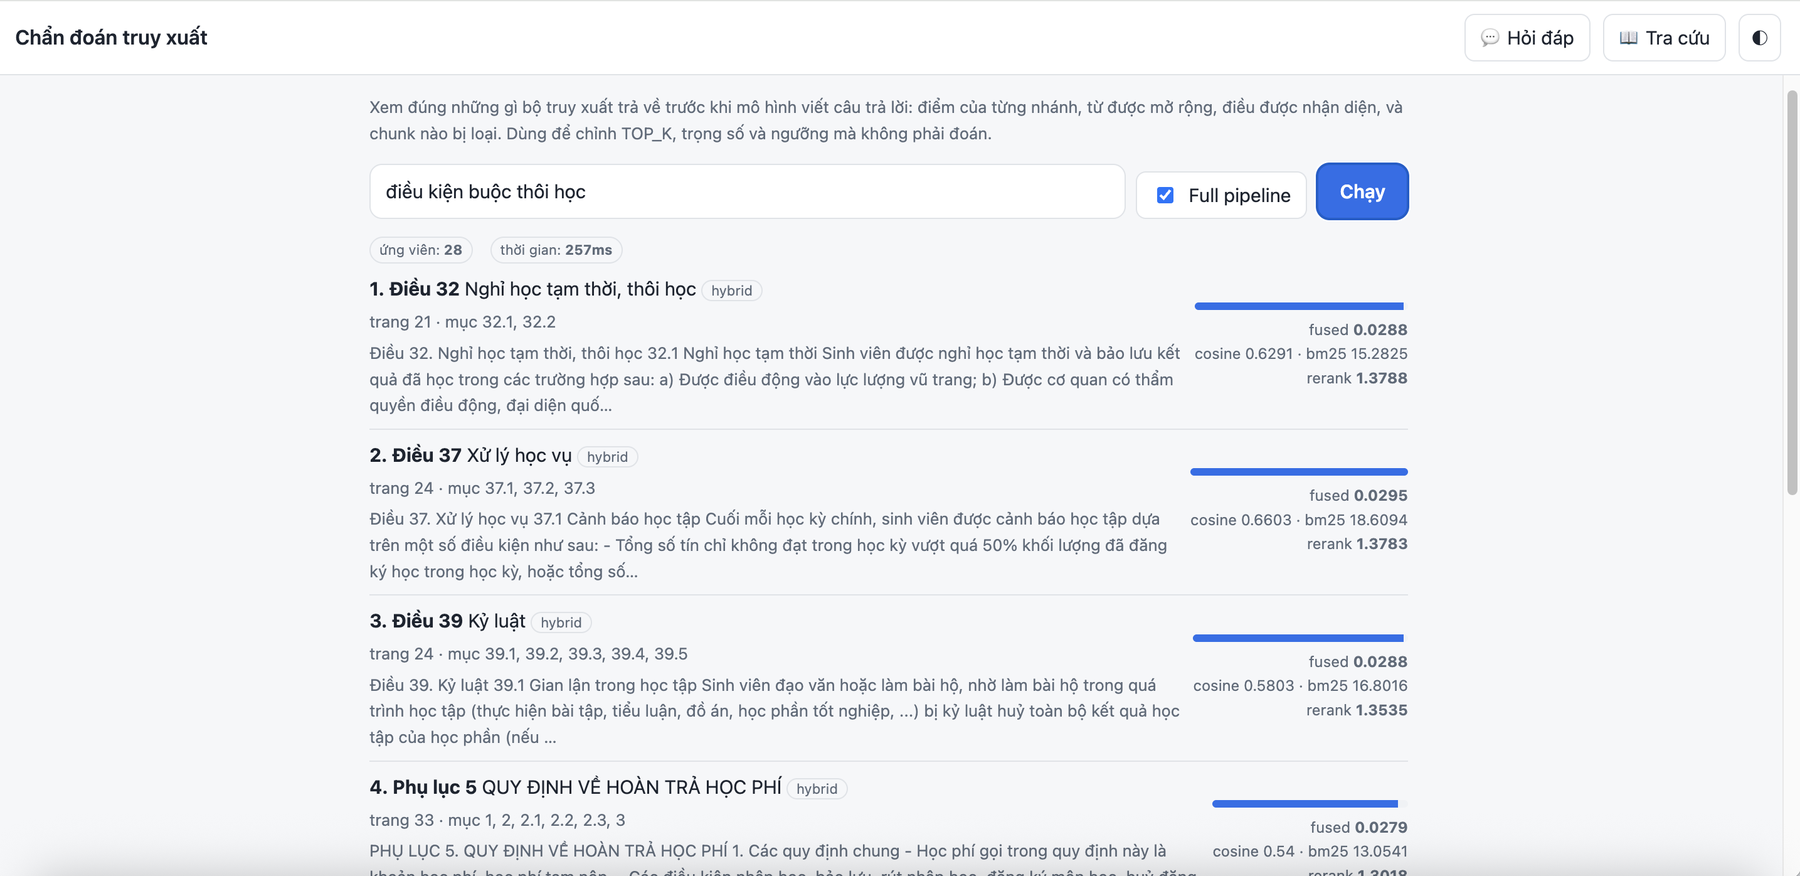
\includegraphics[width=\textwidth]{img/debug-real.png}
\caption{Trang chẩn đoán với câu hỏi “điều kiện buộc thôi học”: 28 ứng viên, 257\,ms, kèm điểm
của từng nhánh cho mỗi chunk.}
\label{fig:debug}
\end{figure}

Điều 37 (Xử lý học vụ) có cosine cao nhất (0,6603) và BM25 cao nhất (18,61), nhưng Điều 32 mới
lên hạng nhất sau rerank — cả hai đều đúng chủ đề. Chính dạng thông tin tách bạch từng nhánh
này cho phép tinh chỉnh trọng số dựa trên quan sát thay vì phỏng đoán.

\subsection{Thống kê kho dữ liệu}

\begin{rtable}
\begin{tabularx}{\textwidth}{@{}X r@{}}
\toprule
\textbf{Chỉ số} & \textbf{Giá trị} \\
\midrule
Số văn bản & 1 \\
Số trang PDF gốc (bản quét, 19\,MB) & 57 \\
Số chương / điều / phụ lục & 10 / 42 / 15 \\
Số chú thích lề tách được & 77 \\
Số chunk sinh ra & 90 \\
Token mỗi chunk: nhỏ nhất / trung vị / lớn nhất & 56 / 508 / 822 \\
Số chunk vượt ngưỡng 800 token (đều là bảng) & 1 \\
Độ dài trung bình (âm tiết mỗi chunk) & 372 \\
Số chunk mang chú thích nguồn gốc & 60 / 90 \\
Số chunk chứa bảng biểu & 18 / 90 \\
\bottomrule
\end{tabularx}
\captionof{table}{Thống kê kho dữ liệu sau khi nạp.}
\label{tab:corpus}
\end{rtable}

Chỉ một chunk vượt ngưỡng token, và đó là một bảng — đúng theo thiết kế, vì bảng không bao giờ
bị cắt. Trung vị 508 token cho thấy phần lớn các Điều vừa trọn trong một chunk.

\subsection{Kết quả đánh giá truy xuất}

Bộ câu hỏi vàng gồm 30 câu trải khắp văn bản, mỗi câu kèm (các) Điều thực sự trả lời được.
Harness bật dần từng kỹ thuật, bắt đầu từ chỉ dùng dense:

\begin{figure}[htbp]
\centering
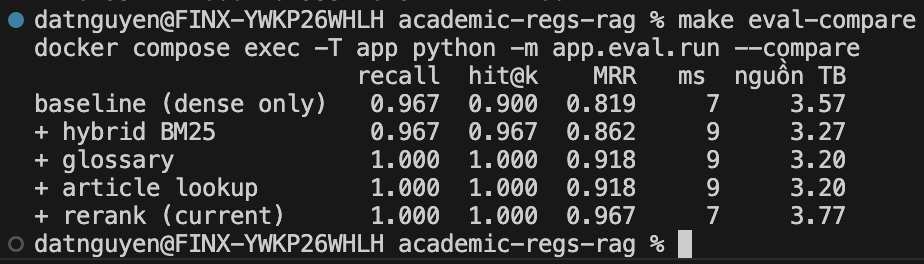
\includegraphics[width=0.84\textwidth]{img/eval-compare.png}
\caption{Kết quả \code{make eval-compare} trên hệ thống thật (bge-m3 + Qdrant), 30 câu hỏi
vàng.}
\label{fig:evalcompare}
\end{figure}

\begin{rtable}
\begin{tabular}{@{}p{0.23\textwidth} r r r r r p{0.22\textwidth}@{}}
\toprule
\textbf{Cấu hình} & \textbf{recall@20} & \textbf{hit@5} & \textbf{MRR} & \textbf{ms}
  & \textbf{nguồn TB} & \textbf{Đóng góp} \\
\midrule
Chỉ dense          & 0,967 & 0,900 & 0,819 & 7 & 3,57 & Nền tảng \\
+ hybrid BM25      & 0,967 & 0,967 & 0,862 & 9 & 3,27 & hit@5 +6,7 điểm \\
+ glossary         & 1,000 & 1,000 & 0,918 & 9 & 3,20 & recall về 100\% \\
+ tra theo số điều & 1,000 & 1,000 & 0,918 & 9 & 3,20 & không đổi trên bộ này \\
\textbf{+ rerank (hiện tại)} & \textbf{1,000} & \textbf{1,000} & \textbf{0,967} & 7 & 3,77
  & MRR +0,049 \\
\bottomrule
\end{tabular}
\captionof{table}{Đóng góp của từng kỹ thuật. \code{recall@20}: Điều đúng có mặt trong danh
sách ứng viên. \code{hit@5}: Điều đúng sống sót qua ngưỡng, rerank và lát cắt cuối. \code{MRR}:
nghịch đảo thứ hạng của Điều đúng. Cột \code{ms} là thời gian truy xuất, không tính lần
embedding đầu tiên vì bộ nhớ đệm đã ấm sau lượt chạy trước.}
\label{tab:eval}
\end{rtable}

Đọc bảng này cho thấy bốn điều mà cảm tính không nói được:

\begin{itemize}
  \item \textbf{BM25 không cải thiện recall mà cải thiện thứ hạng.} Cả hai cấu hình đầu đều tìm
  ra 29/30 Điều đúng ở đâu đó trong 20 ứng viên; khác biệt nằm ở chỗ BM25 đẩy Điều đúng lên đủ
  cao để lọt vào lát cắt cuối (hit@5 từ 0,900 lên 0,967).
  \item \textbf{Bảng thuật ngữ bịt nốt lỗ hổng cuối.} Câu hỏi duy nhất mà hai cấu hình đầu bỏ
  sót là câu gõ không dấu; mở rộng thuật ngữ đưa recall và hit@5 lên 100\%.
  \item \textbf{Tra theo số điều không đóng góp gì trên bộ câu hỏi này}, vì chỉ có một câu gọi
  tên điều khoản và tìm kiếm vector vốn đã tìm ra. Đây là cơ chế \emph{bảo hiểm}: nó bảo đảm
  câu hỏi dạng “Điều 15 nói gì?” không bao giờ hỏng, chứ không phải để nâng điểm trung bình.
  Giữ lại một kỹ thuật không làm tăng điểm là quyết định có ý thức, và bảng đo là thứ cho phép
  đưa ra quyết định đó một cách minh bạch.
  \item \textbf{Rerank đẩy MRR lên 0,967} — gần như lúc nào Điều đúng cũng ở vị trí đầu tiên.
  Với người dùng, điều này quyết định trích đoạn nào được mô hình đọc trước và trích dẫn.
\end{itemize}

\subsubsection{Tinh chỉnh ngưỡng liên quan tương đối}
\label{sec:sweep}

Mục~\ref{sec:nguong} nêu rằng \code{RELATIVE\_CUTOFF} phải đo trên mô hình thật chứ không đoán,
vì siết quá tay sẽ loại nhầm Điều đúng. Harness có chế độ \code{--sweep} in ra chính đường
đánh đổi đó:

\begin{figure}[htbp]
\centering
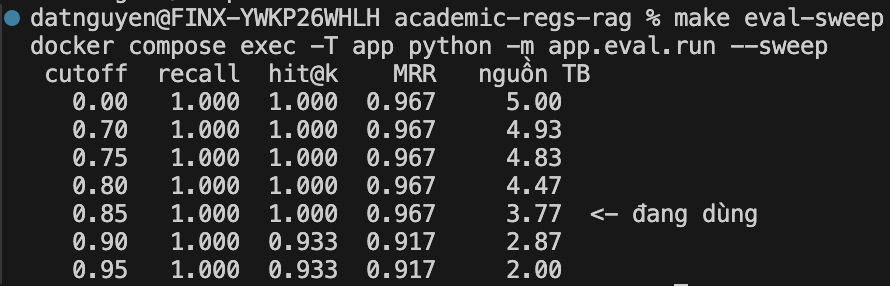
\includegraphics[width=0.80\textwidth]{img/eval-sweep.png}
\caption{\code{make eval-sweep}: số nguồn hiển thị giảm dần khi siết ngưỡng, và điểm gãy nằm ở
0,90.}
\label{fig:evalsweep}
\end{figure}

\begin{rtable}
\begin{tabular}{@{}r r r r r p{0.36\textwidth}@{}}
\toprule
\textbf{cutoff} & \textbf{recall} & \textbf{hit@5} & \textbf{MRR} & \textbf{nguồn TB}
  & \textbf{Nhận xét} \\
\midrule
0,00 & 1,000 & 1,000 & 0,967 & 5,00 & Không lọc: luôn trả đủ định mức \\
0,70 & 1,000 & 1,000 & 0,967 & 4,93 & Gần như không lọc được gì \\
0,75 & 1,000 & 1,000 & 0,967 & 4,83 & \\
0,80 & 1,000 & 1,000 & 0,967 & 4,47 & \\
\textbf{0,85} & \textbf{1,000} & \textbf{1,000} & \textbf{0,967} & \textbf{3,77}
  & \textbf{Đang dùng: bớt 25\% số nguồn mà không mất gì} \\
0,90 & 1,000 & 0,933 & 0,917 & 2,87 & Điểm gãy: bắt đầu loại nhầm Điều đúng \\
0,95 & 1,000 & 0,933 & 0,917 & 2,00 & Quá chặt \\
\bottomrule
\end{tabular}
\captionof{table}{Đường đánh đổi của \code{RELATIVE\_CUTOFF} trên 30 câu hỏi vàng.}
\label{tab:sweep}
\end{rtable}

Kết quả cho thấy giá trị 0,85 là \textbf{miễn phí}: \code{hit@5} và \code{MRR} giữ nguyên hệt
như khi không lọc, trong khi số trích đoạn trung bình đưa ra cho người đọc giảm từ 5,00 xuống
3,77 — tức một phần tư số “nguồn tham khảo” trước đây là phần đệm không đóng góp gì. Điểm gãy
nằm ở 0,90, nơi \code{hit@5} tụt xuống 0,933. Đây đúng là dạng quyết định mà nếu không có công
cụ đo thì chỉ còn cách chọn bừa một con số rồi hy vọng.

\subsection{Kiểm thử tự động}

\begin{rtable}
\begin{tabular}{@{}p{0.24\textwidth} r p{0.55\textwidth}@{}}
\toprule
\textbf{Tệp} & \textbf{Test} & \textbf{Kiểm tra điều gì} \\
\midrule
\code{test\_chunk.py} & 9 & Mọi Điều/Phụ lục đều có chunk; chỉ bảng được vượt ngưỡng; mã chunk tất định \\
\code{test\_retriever.py} & 17 & Hợp nhất giữ điểm từng nhánh; tra theo số điều; ngưỡng liên quan; mở rộng lân cận; số nguồn biến thiên \\
\code{test\_chat.py} & 14 & Thứ tự sự kiện SSE; đường từ chối; soát trích dẫn; bộ bảo vệ rewrite \\
\code{test\_api.py} & 10 & Mục lục, đọc Điều, cấu hình không lộ khoá, chống path traversal \\
\code{test\_glossary.py} & 7 & Viết tắt, tiếng lóng, không dấu, viết tắt 2 ký tự phải hoa \\
\code{test\_rerank.py} & 7 & IDF cục bộ; độ phủ; chunk hạng thấp được nâng lên; phạt trùng Điều \\
\code{test\_citations.py} & 5 & Bắt số Điều/khoản/Phụ lục; phát hiện trích dẫn vô căn cứ \\
\midrule
\textbf{Tổng} & \textbf{69} & Chạy trong khoảng một giây, không cần Ollama, Qdrant hay mạng \\
\bottomrule
\end{tabular}
\captionof{table}{Bộ kiểm thử tự động.}
\label{tab:tests}
\end{rtable}

Việc bộ test chạy được mà không cần hạ tầng là một quyết định thiết kế chứ không phải tiện lợi
ngẫu nhiên: Qdrant có chế độ in-memory, và embedder được thay bằng một bộ băm túi từ tất định.
Bộ test nào cần dựng cả stack mới chạy được thì sẽ không ai chạy.

\subsection{Hiệu năng}

\begin{rtable}
\begin{tabularx}{\textwidth}{@{}X r@{}}
\toprule
\textbf{Giai đoạn} & \textbf{Thời gian đo được} \\
\midrule
Truy xuất (hybrid + rerank + mở rộng) & 11 – 340\,ms \\
Toàn bộ một lượt hỏi đáp (gpt-4o-mini) & 2,4 – 6,1\,s \\
Lượt bị từ chối (không gọi mô hình sinh) & 1,3\,s \\
Nạp dữ liệu lại toàn bộ 90 chunk (CPU) & vài phút \\
Nạp dữ liệu khi không có thay đổi & tức thì \\
\bottomrule
\end{tabularx}
\captionof{table}{Hiệu năng đo trên máy thật, chế độ cloud (\code{--cloud}, embedding vẫn
chạy local).}
\label{tab:perf}
\end{rtable}

Độ trễ tổng bị chi phối hoàn toàn bởi bước sinh câu trả lời; phần truy xuất chiếm chưa tới
10\%. Đây là lý do việc gửi trích đoạn trước token đầu tiên (mục~\ref{sec:latency}) có giá trị
thực tế: người đọc nhận được nội dung kiểm chứng được sau khoảng 300\,ms, thay vì phải chờ hết
vài giây.

\chapterbreak

\section{Đánh giá và hạn chế}

\subsection{Đối chiếu với mục tiêu}

\begin{rtable}
\begin{tabular}{@{}p{0.26\textwidth} p{0.10\textwidth} p{0.52\textwidth}@{}}
\toprule
\textbf{Yêu cầu} & \textbf{Kết quả} & \textbf{Bằng chứng} \\
\midrule
Chỉ trả lời dựa trên văn bản & Đạt & Prompt ràng buộc + soát trích dẫn tự động; hình~\ref{fig:count} cho thấy đường từ chối hoạt động \\
Truy vết được & Đạt & Trích dẫn bấm được (hình~\ref{fig:chat1}), mở trích đoạn gốc (hình~\ref{fig:source}), mở PDF đúng trang \\
Biết nói “không biết” & Đạt & Ngưỡng liên quan theo từng trích đoạn + câu trả lời cố định \\
Chạy tại chỗ & Đạt & Ollama + Qdrant trong Docker; chế độ cloud là tuỳ chọn, embedding luôn local \\
Chất lượng đo được & Đạt & hit@5 = 1,000 và MRR = 0,967 trên 30 câu hỏi vàng (bảng~\ref{tab:eval}) \\
\bottomrule
\end{tabular}
\captionof{table}{Đối chiếu kết quả với yêu cầu ban đầu.}
\label{tab:doichieu}
\end{rtable}

\subsection{Hạn chế}

\begin{itemize}
  \item \textbf{Bộ câu hỏi vàng do nhóm tự soạn.} 30 câu là nhỏ, và quan trọng hơn, chúng được
  viết bởi người đã đọc văn bản — nên có thiên lệch về từ ngữ so với câu hỏi thật của sinh
  viên. Con số hit@5 = 1,000 vì vậy nên đọc là “không còn lỗ hổng rõ ràng nào trên tập này”,
  chứ không phải “hệ thống không bao giờ trượt”.
  \item \textbf{Chưa đánh giá chất lượng câu trả lời.} Harness đo truy xuất, không đo phần
  sinh. Việc mô hình có diễn giải trung thực trích đoạn hay không hiện chỉ được kiểm bằng mắt
  và bởi cơ chế soát trích dẫn.
  \item \textbf{Phụ thuộc bước rà soát thủ công.} Chất lượng toàn hệ thống bị chặn trên bởi
  chất lượng bản Markdown sau OCR. Với văn bản 57 trang thì chấp nhận được; mở rộng ra hàng
  chục văn bản thì đây là nút thắt.
  \item \textbf{Một văn bản duy nhất.} Pipeline hỗ trợ đa tài liệu nhưng chưa được kiểm chứng ở
  quy mô đó. Khi có nhiều văn bản chồng lấn (quy định cũ – mới), sẽ phát sinh bài toán mới: ưu
  tiên văn bản còn hiệu lực.
  \item \textbf{Endpoint \code{/ingest} chưa xác thực.} Ai truy cập được cổng đều kích hoạt
  được việc nạp lại dữ liệu. Chấp nhận được khi chạy localhost, phải khoá lại nếu triển khai
  thật.
  \item \textbf{\code{/chat} là endpoint đồng bộ}, chạy trong threadpool của FastAPI. Với vài
  chục người dùng đồng thời cần chuyển sang I/O bất đồng bộ.
\end{itemize}

\subsection{Bài học}

Bốn lỗi đáng nhớ nhất trong quá trình làm, đều cùng một kiểu: \emph{trông thì đúng}.

\begin{enumerate}
  \item \textbf{Chuẩn hoá min–max trong bộ rerank.} Nó ánh xạ ứng viên tốt nhất về 1 và kém
  nhất về 0, khiến hai ứng viên chênh nhau 0,01 trông xa nhau như 1,0 và 0,0, và mọi tín hiệu
  từ vựng trở nên vô dụng. Phát hiện nhờ một unit test, không phải nhờ đọc code.
  \item \textbf{Cướp câu hỏi ở bước viết lại} (mục~\ref{sec:rewrite}, hình~\ref{fig:bug}). Hệ
  thống trả lời sai chủ đề nhưng với trích dẫn thật — không một chỉ số kỹ thuật nào bắt được,
  chỉ phát hiện khi có người gõ một câu hỏi vu vơ.
  \item \textbf{Ngưỡng liên quan dùng như một cánh cổng chung} (mục~\ref{sec:nguong}). Chỉ cần
  một trích đoạn đúng là cả năm trích đoạn top-k được giữ theo, nên mọi câu trả lời đều kèm
  đúng từng ấy “nguồn tham khảo” — kể cả câu trả lời kết luận là không tìm thấy gì. Không test
  nào bắt được, vì hệ thống chạy đúng như code mô tả; chỉ người dùng để ý thấy con số không bao
  giờ đổi mới phát hiện ra.
  \item \textbf{Tên file tiếng Việt trong HTTP header.} Header HTTP chỉ mã hoá được latin-1;
  tên file tiếng Việt làm máy chủ trả lỗi 500 khi mở PDF. Kèm theo đó là một lỗi tiềm ẩn: macOS
  lưu tên file ở dạng NFD còn siêu dữ liệu ghi dạng NFC — hai chuỗi như nhau trên macOS nhưng
  khác nhau trong container Linux.
\end{enumerate}

Mẫu số chung: lỗi nguy hiểm nhất của một hệ thống RAG không phải lỗi làm nó hỏng, mà lỗi làm nó
trả lời \textbf{tự tin và sai}, hoặc trình bày thứ trông như bằng chứng mà thực ra không phải.
Đó là lý do đồ án đầu tư vào ba lớp phòng thủ — ngưỡng liên quan theo từng trích đoạn, soát
trích dẫn, và bộ bảo vệ bước viết lại — thay vì chỉ tối ưu điểm số.

\chapterbreak

\section{Hướng phát triển}

\begin{enumerate}
  \item \textbf{Mở rộng kho văn bản} sang quy chế công tác sinh viên, quy định học phí từng
  năm, thông báo học vụ. Cần bổ sung cơ chế đánh dấu hiệu lực để không trả lời bằng văn bản đã
  hết hạn.
  \item \textbf{Đánh giá phần sinh câu trả lời}, không chỉ truy xuất: xây bộ đối chiếu câu hỏi
  – đáp án chuẩn và chấm bằng mô hình mạnh hơn hoặc bằng người.
  \item \textbf{Chuyển \code{/chat} sang bất đồng bộ} và thêm giới hạn tần suất, điều kiện cần
  trước khi mở cho toàn trường.
  \item \textbf{Bộ nhớ đệm câu trả lời theo ngữ nghĩa.} Hiện mới đệm vector câu hỏi; với một
  kho câu hỏi lặp lại cao như học vụ, đệm cả câu trả lời sẽ giảm mạnh chi phí.
  \item \textbf{Vòng lặp cải thiện từ dữ liệu thật.} Nhật ký truy vấn và nút phản hồi đã sẵn
  sàng; việc còn lại là định kỳ lấy các câu bị đánh giá kém hoặc không trả lời được, bổ sung
  vào bộ câu hỏi vàng và bảng thuật ngữ.
  \item \textbf{Tích hợp dữ liệu cá nhân} (điểm, số tín chỉ tích luỹ) để trả lời được “em còn
  thiếu gì để tốt nghiệp?”. Đây là bước đổi về chất, kéo theo yêu cầu xác thực và bảo mật.
\end{enumerate}

\chapterbreak

\section{Kết luận}

Đồ án đã xây dựng hoàn chỉnh một hệ thống RAG tiếng Việt chạy tại chỗ cho bài toán tra cứu quy
định học vụ, gồm 33 chức năng, khoảng 3.700 dòng Python và 1.000 dòng giao diện, được bảo vệ
bởi 69 test tự động và một bộ đánh giá truy xuất 30 câu hỏi.

Kết quả đo được trên hệ thống thật: Điều đúng xuất hiện trong danh sách ứng viên ở
\textbf{100\%} số câu hỏi, sống sót qua toàn bộ pipeline để vào prompt ở \textbf{100\%}, và
đứng ở vị trí đầu tiên trong hầu hết các trường hợp (\textbf{MRR = 0,967}). So với cấu hình chỉ
dùng tìm kiếm vector, hit@5 tăng từ 0,900 lên 1,000 và MRR tăng từ 0,819 lên 0,967. Ngưỡng liên
quan tương đối còn cắt được một phần tư số trích đoạn thừa mà không mất một điểm chất lượng
nào.

Điều nhóm cho là đáng giá nhất lại không phải các con số đó. Với một hệ thống tra cứu văn bản
quy phạm, giá trị nằm ở chỗ người đọc \emph{kiểm chứng được} và hệ thống \emph{biết im lặng
đúng lúc}: mỗi ý đều mở được ra đúng đoạn văn bản gốc và đúng trang PDF, trích dẫn không có căn
cứ bị đánh dấu, và câu hỏi ngoài phạm vi nhận một lời từ chối thay vì một câu trả lời trôi
chảy. Bốn chế độ hỏng được ghi lại ở mục~\ref{sec:chitiet} và phần bài học cho thấy đây không
phải mối lo lý thuyết — cả bốn đều là lỗi khiến hệ thống trả lời tự tin và sai, và đều chỉ lộ
ra khi có cơ chế đo đạc hoặc có người thật gõ một câu hỏi thật.

\chapterbreak

\section*{Tài liệu tham khảo}
\addcontentsline{toc}{section}{Tài liệu tham khảo}
\markboth{Tài liệu tham khảo}{}

\begin{thebibliography}{99}
\setlength{\itemsep}{0.35em}

\bibitem{lewis2020} P. Lewis và cộng sự. \emph{Retrieval-Augmented Generation for
Knowledge-Intensive NLP Tasks}. NeurIPS, 2020.

\bibitem{bm25} S. Robertson và H. Zaragoza. \emph{The Probabilistic Relevance Framework: BM25
and Beyond}. Foundations and Trends in Information Retrieval, 3(4), 2009.

\bibitem{rrf} G. V. Cormack, C. L. A. Clarke và S. Buettcher. \emph{Reciprocal Rank Fusion
Outperforms Condorcet and Individual Rank Learning Methods}. SIGIR, 2009.

\bibitem{bgem3} J. Chen và cộng sự. \emph{BGE M3-Embedding: Multi-Lingual, Multi-Functionality,
Multi-Granularity Text Embeddings Through Self-Knowledge Distillation}. BAAI, 2024.

\bibitem{xlmr} A. Conneau và cộng sự. \emph{Unsupervised Cross-lingual Representation Learning
at Scale} (XLM-RoBERTa). ACL, 2020.

\bibitem{qdrant} Qdrant. \emph{Hybrid Search and Sparse Vectors — Documentation}.
\url{https://qdrant.tech/documentation}

\bibitem{ollama} Ollama. \emph{OpenAI-compatible API — Documentation}.
\url{https://ollama.com/blog/openai-compatibility}

\bibitem{quydinh} Trường Đại học Bách khoa – ĐHQG-HCM. \emph{Quy định về học vụ và đào tạo bậc
đại học – Phiên bản hợp nhất}, số 285/ĐHBK-ĐT ngày 28/7/2022.

\bibitem{tt0817} Bộ Giáo dục và Đào tạo. \emph{Thông tư 08/2021/TT-BGDĐT} ban hành Quy chế đào
tạo trình độ đại học; \emph{Thông tư 17/2021/TT-BGDĐT} quy định về chuẩn chương trình đào tạo.

\end{thebibliography}

\chapterbreak

\appendix
% Phụ lục đánh A, B, C và hiện đủ chữ "Phụ lục" cả ở tiêu đề lẫn mục lục.
\renewcommand{\thesection}{Phụ lục~\Alph{section}}
\setcounter{section}{0}
\addtolength{\cftsecnumwidth}{3.4em}

\section{Cấu trúc mã nguồn}

\begin{codeblock}
academic-regs-rag/
├── app/
│   ├── config.py              cấu hình từ biến môi trường, có kiểu
│   ├── api/
│   │   ├── main.py            15 endpoint HTTP, luồng SSE
│   │   ├── library.py         đọc văn bản: mục lục, toàn văn một Điều, PDF gốc
│   │   └── telemetry.py       nhật ký truy vấn và phản hồi, thống kê sử dụng
│   ├── ingest/
│   │   ├── ocr.py             OCR hai độ phân giải, tách chú thích lề
│   │   ├── parse.py           PDF có text layer / DOCX / TXT -> Markdown
│   │   ├── chunk.py           phân mảnh bám cấu trúc Chương -> Điều -> khoản
│   │   └── run.py             nạp dữ liệu tăng dần, manifest, dấu vân tay
│   ├── rag/
│   │   ├── glossary.py        mở rộng thuật ngữ, xử lý câu hỏi không dấu
│   │   ├── citations.py       bắt số Điều trong câu hỏi, soát trích dẫn
│   │   ├── embeddings.py      dense qua Ollama + BM25 cho tiếng Việt
│   │   ├── store.py           Qdrant: schema, truy vấn theo lô, lọc payload
│   │   ├── retriever.py       mở rộng -> tìm -> hợp nhất -> rerank -> ngữ cảnh
│   │   ├── rerank.py          rerank heuristic + rerank bằng LLM (tuỳ chọn)
│   │   ├── prompt.py          prompt tiếng Việt, lắp ngữ cảnh theo ngân sách
│   │   ├── llm.py             client tương thích OpenAI, lọc khối <think>
│   │   └── chat.py            một lượt hỏi đáp dưới dạng luồng sự kiện
│   ├── eval/
│   │   ├── questions.toml     30 câu hỏi vàng
│   │   └── run.py             đo recall@k / hit@final / MRR, chế độ sweep
│   └── static/
│       ├── index.html         trang hỏi đáp
│       ├── browse.html        trang tra cứu toàn văn
│       ├── debug.html         trang chẩn đoán truy xuất
│       └── style.css          giao diện dùng chung, sáng/tối
├── tests/                     69 test, không cần Ollama/Qdrant
├── data/
│   ├── raw/                   PDF gốc
│   ├── processed/             Markdown đã rà soát  <- nguồn chân lý
│   └── logs/                  nhật ký truy vấn, phản hồi
├── docs/report/               mã nguồn LaTeX của báo cáo này
├── docker-compose.yml         ba dịch vụ, healthcheck, volume
├── start.sh / start.ps1       một lệnh từ bản sao sạch tới hệ thống chạy được
├── Makefile                   up · ingest · test · eval · eval-sweep · metrics
└── README.md, docs/architecture.md
\end{codeblock}

\section{Danh mục API}

{\sffamily\small
\begin{longtable}{@{}p{0.08\textwidth} p{0.27\textwidth} p{0.55\textwidth}@{}}
\caption{Danh mục API.}\label{tab:api}\\
\toprule
\textbf{Method} & \textbf{Đường dẫn} & \textbf{Chức năng} \\
\midrule
\endfirsthead
\toprule
\textbf{Method} & \textbf{Đường dẫn} & \textbf{Chức năng} \\
\midrule
\endhead
\bottomrule
\endlastfoot
GET  & \code{/} & Trang hỏi đáp \\
GET  & \code{/browse} & Trang tra cứu toàn văn \\
GET  & \code{/debug} & Trang chẩn đoán truy xuất \\
POST & \code{/chat} & Một lượt hỏi đáp, trả về luồng SSE: \code{query? → retrieved → token* → sources → done} \\
GET  & \code{/search} & Kết quả truy xuất kèm điểm từng nhánh; \code{final=true} chạy đủ pipeline \\
GET  & \code{/toc} & Mục lục mọi văn bản đã nạp \\
GET  & \code{/article} & Toàn văn một Điều/Phụ lục, tách theo khoản \\
GET  & \code{/source/\{doc\_id\}} & PDF gốc, mở inline để nhảy tới \code{\#page=N} \\
POST & \code{/feedback} & Ghi nhận phản hồi kèm câu hỏi và nguồn đã dùng \\
GET  & \code{/metrics} & Tỉ lệ trả lời được, độ trễ p50/p95, câu hỏi không có đáp án \\
GET  & \code{/config} & Tham số truy xuất đang áp dụng (không chứa khoá bí mật) \\
GET  & \code{/health} & Ollama, model, Qdrant, dữ liệu — 200 hoặc 503 kèm lý do \\
GET  & \code{/livez} & Tiến trình còn sống (healthcheck của container) \\
POST & \code{/ingest} & Kích hoạt nạp dữ liệu chạy nền \\
GET  & \code{/ingest} & Trạng thái lần nạp gần nhất \\
\end{longtable}
}

\section{Biên dịch báo cáo}

Mã nguồn LaTeX của báo cáo nằm trong \code{docs/report/}. Bắt buộc dùng XeLaTeX vì báo cáo dùng
font hệ thống và tiếng Việt Unicode.

\begin{codeblock}
cd docs/report
./build.sh            # dùng xelatex nếu máy đã cài, nếu không thì dùng Docker
\end{codeblock}


\end{document}
